\documentclass{article}

\usepackage{enumerate}
\usepackage{amsmath, amsthm}
\usepackage{amssymb}
\usepackage{bbm}
\usepackage{graphicx}
\usepackage[english]{babel}
\usepackage[letterpaper, portrait, margin=1.0in]{geometry}
\graphicspath{ {~/Desktop/Uchicago/STAT_347/HW/HW2/QuestionA3} }
\usepackage{mathrsfs}
\usepackage{breqn}
\usepackage{mathtools}
\usepackage{rotating}
\usepackage{bm}
\usepackage{txfonts}
\DeclarePairedDelimiter\ceil{\lceil}{\rceil}
\DeclarePairedDelimiter\floor{\lfloor}{\rfloor}
\usepackage{units}
\DeclareMathOperator{\Tr}{Tr}
\DeclareMathOperator{\diag}{diag}
\DeclareMathOperator*{\argmin}{arg\,min}
\DeclareMathOperator*{\argmax}{arg\,max}
\usepackage{setspace}
\newcommand{\indep}{\rotatebox[origin=c]{90}{$\models$}}
\DeclareMathOperator{\E}{\mathbb{E}}
\DeclarePairedDelimiter\abs{\lvert}{\rvert}%
\DeclarePairedDelimiter\norm{\lVert}{\rVert}%


% Swap the definition of \abs* and \norm*, so that \abs
% and \norm resizes the size of the brackets, and the 
% starred version does not.
\makeatletter
\let\oldabs\abs
\def\abs{\@ifstar{\oldabs}{\oldabs*}}
%
\let\oldnorm\norm
\def\norm{\@ifstar{\oldnorm}{\oldnorm*}}
\makeatother

\newtheorem{theorem}{Theorem}[section]
\newtheorem{corollary}{Corollary}[theorem]
\newtheorem{lemma}[theorem]{Lemma}
 

\begin{document}


\section*{Outline}
\begin{enumerate}
\item Write out and talk about model for the data (maybe discuss M vs. Beta value here)
\item Discuss methods without cell type data (i.e. Houseman and CATE).
\item When do these perform well?
	\begin{enumerate}
	\item Standardized effect size for $L$, taking into account variability $\Xi$.
	\item Discuss $\frac{1}{p}\Gamma^T \Sigma^{-1}\Gamma$ result in Bai and Li, i.e. how informative methylation data are for cell type.
	\item Figures: simulation results. We will ALWAYS underestimate $\Omega$ when data are not informative. Effect on results is small when $\Omega$ is small (can we prove this?)
	\item Give Amish/Hutterite data example. Talk about size of $\frac{1}{p}\Gamma^T \Sigma^{-1}\Gamma$, MAJOR differences in the estimates for $\pi_0$, the fact that the data suggest that there is confounding (p-value for $\alpha$). Large difference in $\hat{\pi}_0$ along with the fact that $\frac{1}{p}\Gamma^T \Sigma^{-1}\Gamma = O\left( \frac{1}{n} \right)$ seem to indicate the data are not informative enough to estimate the correlation between $C$ and $X$. 
	\end{enumerate}
\item If data are not informative for cell type, we need another method to estimate the correlation between $C$ and $X$. Obvious alternative: collect cell type or use training data to estimate the correlation between $C$ and $X$.
\item In some circumstances, we can do well with only partially observed data (in the absence of other confounders). Plot simulation figures. When does this happen? What happens when we have additional confounders?
\item Recommendations: if you have strong prior assumptions that there are additional confounders that you can measure, it is always a good idea to measure them.
	\begin{enumerate}
	\item Talk about how large correlation needs to be to start making serious errors. If standardized correlation is small, maybe you don't need to worry about it and can estimate it from the data.
	\item With strong prior knowledge, it is always a good idea to include covariates that may have an effect on response and are correlated with the variable of interest.
	\end{enumerate}
\end{enumerate}

\section{Notation}
\begin{itemize}
\item All matrices (including vectors) are bold and all vectors are column vectors, unless otherwise stated.
\item Throughout the paper, the matrix $\bm{X} = \bm{X}_{d \times n} \in \mathbb{R}^{d \times n}$ contains $d$ covariates of interest (including an intercept) measured on $n$ individuals. For example, in the real data example $d = 2$ where one covariate is the intercept and the other is the Amish vs. Hutterite contrast.
\item Cell type proportions for $K$ cells measured on $n$ individuals is given as the matrix $\bm{C} = \bm{C}_{K \times n} \in [0-1]^{K \times n}$.
\item $P_{\bm{A}}$ is the orthogonal projection onto the linear subspace generated by the columns of $\bm{A}$ and $P_{\bm{A}}^{\perp}$ projects onto the subspace orthogonal to $\text{Image}\left( \bm{A} \right)$.
\item $\text{vec}\left( \bm{A} \right)$ is the vectorized version of a matrix, obtain by column stacking.
\item When the matrix $\bm{U} \in \mathbb{R}^{p x n}$ is random and the covariance of the elements of $\bm{U}$ are separable across rows and columns, we will write
\[
\bm{U} \sim \left( \bm{\mu}_{p \times n}, \left[ \bm{S}_{p \times p}, \bm{R}_{n \times n} \right] \right)
\]
to indicate that $\bm{\mu}$ is the mean of $\bm{U}$, $\bm{S}$ is the covariance across rows and $\bm{R}$ is the covariance across columns. That is, $\text{Var}\left( \text{vec}\left( \bm{U} \right) \right) = \bm{R} \otimes \bm{S}$. For example, if we measured the methylation on $p$ CpG sites across $n$ independent individuals, $\bm{R} = I_n$ and $\bm{S}$ would be the covariance across the $p$ CpG sites in a single sample. We characterize random variables by their first two moments, as it is often times more important to accurately estimate the mean and variance than it is to use the correct probability model (cite contiguity paper).

\end{itemize}

\section{The Model}
Let $\bm{Y}_{p \times n}$ be the methylation response measured on $p$ CpG sites across $n$ independent individuals, $\bm{X}_{d \times n} = \left[ \begin{matrix}
\vec{x}_1 & \cdots & \vec{x}_n
\end{matrix} \right]$ the matrix of $d$ covariates of interest (i.e. disease status, sex, etc.) measured on the same $n$ individuals and $\bm{C}_{K \times n} = \left[ \begin{matrix}
\vec{c}_1 & \cdots & \vec{c}_n
\end{matrix} \right]$ be the cell composition matrix for $K$ cell types across the $n$ individuals  Assuming that methylation status is ONLY affect by the covariate(s) of interest $\bm{X}$ and cell type composition $\bm{C}$, full data model for $\bm{Y}$ is then:
\begin{equation}
\bm{Y}_{p \times n} = \bm{B}_{p \times d}\bm{X}_{d \times n} + \bm{L}_{p \times K}\bm{C}_{K \times n} + \bm{E}_{p \times n}
\end{equation}
Where $\bm{E}_{p \times n} \sim \left( \bm{0}_{p\times n}, \left[\bm{\Sigma}_{p \times p} = \text{diag}\left( \sigma_1^2, \ldots, \sigma_p^2 \right), I_{n}\right] \right)$, $\bm{L} = \left[ \begin{matrix}
\bm{\ell}_1^T\\
\vdots\\
\bm{\ell}_p^T
\end{matrix} \right]$ and $\bm{B} = \left[ \begin{matrix}
\bm{\beta}_1^T\\
\vdots\\
\bm{\beta}_p^T
\end{matrix} \right]$. That is,
\begin{equation}
\bm{Y} \mid \left( \bm{X}, \bm{C} \right) \sim \left( \bm{B}\bm{X} + \bm{L}\bm{C}, \left[\bm{\Sigma}, I_n\right] \right)
\end{equation}
We are interested in estimating the effect $\bm{\beta}_i$ for each CpG site $i = 1, \ldots, p$.\\
\indent However, sometimes we do not have access to the cell type composition data. If cell type is uncorrelated with the covariate(s) of interest, we can account for it using factor analysis correction techniques (e.g. SVA). When cell type and the covariate(s) of interest are correlated, we assume that
\begin{equation}
\bm{C}_{K \times n} = \bm{\Omega}_{K \times d}\bm{X}_{d \times n} + \bm{\Xi}_{K \times n}, \text{, } \bm{\Xi} = \left[ \begin{matrix}
\vec{\xi}_1 & \cdots & \vec{\xi}_n
\end{matrix} \right]
\end{equation}
\begin{equation}
\bm{\Xi} \sim \left( \bm{0}, \left[\Lambda_{K \times K}, I_n\right] \right)
\end{equation}
Note that since cell type composition is proportion data, the variance $E\left( \vec{\xi}_i \vec{\xi}_i^T\mid \vec{x}_i\right)$ is a function of the mean $E\left( \vec{c}_i \mid \vec{x}_i \right)$, which is not captured by our assumptions on $\bm{\Xi}$. We show by simulation that we can ignore the mean-variance relationship and still perform accurate inference on $\hat{\bm{B}}$.\\
\indent When $\bm{C}$ is unobserved, we can write the full data model as
\begin{equation}
\bm{Y} = \bm{B}\bm{X} + \bm{L} \bm{\Omega} \bm{X} + \bm{L}\bm{\Xi} + \bm{E} = \bm{B}\bm{X} + \tilde{\bm{L}} \tilde{\bm{\Omega}} \bm{X} + \tilde{\bm{L}}\tilde{\bm{\Xi}} + \bm{E}
\end{equation}
where $\tilde{\bm{L}} = \left[ \begin{matrix}
\tilde{\bm{\ell}}_1^T\\
\vdots\\
\tilde{\bm{\ell}}_p^T\\
\end{matrix} \right] = L\Lambda^{1/2}$, $\tilde{\Omega} = \Lambda^{-1/2}\Omega$ and $\tilde{\bm{\Xi}} \sim \left( \bm{0}, \left[ I_K, I_n\right] \right)$. The first and second moments conditional on only observing the covariates $\bm{X}$ are
\begin{equation}
\bm{Y} \mid \bm{X} \sim\left( \bm{B}\bm{X} + \tilde{\bm{L}} \tilde{\bm{\Omega}} \bm{X}, \left[\tilde{\bm{L}} \tilde{\bm{L}}^T + \bm{\Sigma}, I_n\right] \right).
\end{equation}



\section{Estimation Methods With Unobserved Cell Type}
We start by assuming $\bm{X}$ and cell type $\bm{C}$ are both observed. We see from equation $\bm{3}$ that if we were to estimate $\tilde{\bm{\Omega}}$ using OLS (assuming $\bm{\Lambda}$ was known), we would get
\begin{equation}
\tilde{\bm{\Omega}}^{(\text{OLS})} = \bm{\Lambda}^{-1/2}\bm{C}\bm{X}^T \left( \bm{X}\bm{X}^T \right)^{-1} = \tilde{\bm{\Omega}} + \tilde{\bm{\Xi}}\bm{X}^T \left( \bm{X}\bm{X}^T \right)^{-1}.
\end{equation} 
Note that there are two sources of empirical correlation. The first is due to the true correlation $\bm{\Omega}$ and the second is due to the residual $\tilde{\bm{\Xi}}\bm{X}^T \left( \bm{X}\bm{X}^T \right)^{-1}$, which we will refer to as spurious correlation. When $\bm{C}$ is observed (i.e. $\bm{\Omega} \bm{X} + \bm{\Xi}$ is observed), the unbiased OLS estimate for $\bm{B}$ is
\begin{equation}
\hat{\bm{B}}^{(\text{OLS})} = \bm{Y} \bm{X}^T \left[ \bm{X}\bm{X}^T \right]^{-1} - \bm{Y} P_{\bm{X}^T}^{\perp} \tilde{\bm{\Xi}}^T \left[ \tilde{\bm{\Xi}} P_{\bm{X}^T}^{\perp}\tilde{\bm{\Xi}}^T \right]^{-1} \tilde{\bm{\Omega}}^{(\text{OLS})} = \bm{Y} \bm{X}^T \left[ \bm{X}\bm{X}^T \right]^{-1} - \hat{\tilde{\bm{L}}}^{(\text{OLS})} \tilde{\bm{\Omega}}^{(\text{OLS})}
\end{equation}
with variance
\begin{equation}
\text{Var}\left( \hat{\bm{\beta}}_i^{(\text{OLS})} \right) = \sigma_i^2\left( \left[ \bm{X}\bm{X}^T \right]^{-1} + \left( \tilde{\bm{\Omega}}^{(\text{OLS})}\right)^T \left[ \tilde{\bm{\Xi}} P_{\bm{X}^T}^{\perp}\tilde{\bm{\Xi}}^T \right]^{-1}\tilde{\bm{\Omega}}^{(\text{OLS})} \right)
\end{equation} 
which by Gauss-Markov is the smallest variance possible among all unbiased estimators for $\bm{\beta}_i$. If cell type $\bm{C}$ is NOT observed, to correct for cell type heterogeneity it stands to reason that our goal should be to estimate the part of $\bm{C}$ uncorrelated with $\bm{X}$ and the part that is correlated with $\bm{X}$. That is, we wish to estimate $P_{\bm{X}^T}^{\perp}\tilde{\bm{\Xi}}^T$ and $\tilde{\bm{\Omega}}^{(\text{OLS})} = $ true correlation $+$ spurious correlation from the methylation data $\bm{Y}$.\\
\indent Luckily, considerable attention has been given to developing methods to estimate $\bm{B}$ in the presence of confounding that is correlated with the design matrix $\bm{X}$ (LEAPP, Houseman et al., CATE). Using \textbf{Equ. 5} as a reference, all three methods assume that $\tilde{\bm{\Xi}}$ is independent of $\bm{X}$ and that $\bm{B}$ is sparse. That is, the covariate of interest affects only a small fraction of the CpG sites. Both of these assumptions tend to hold in real data. To get estimates $\hat{\bm{B}} = \left[ \begin{matrix}
\hat{\bm{\beta}}_1^T\\
\vdots\\
\hat{\bm{\beta}}_p^T
\end{matrix} \right]$ and $\hat{\text{Var}}\left( \hat{\bm{\beta}}_i \right)$ for CpG sites $i = 1, \ldots, p$, all three methods use the following general procedure:
\begin{enumerate}
	\item Compute $\hat{\bm{\tilde{L}}}$ and $\hat{\bm{\Sigma}}$, estimates for $\bm{L}$ and $\bm{\Sigma}$. This is done by regressing out $\bm{X}$ from \textbf{Equ. 5} and then performing factor analysis on the residual matrix $\bm{Y}P_{X^T}^{\perp}$.
	\item Compute $\hat{\tilde{\bm{\Xi}}}^{\perp}$, an estimate for $\tilde{\bm{\Xi}} P_{X^T}^{\perp}$. Two possibilities for $\hat{\tilde{\bm{\Xi}}}^{\perp}$ are the BLUP for $\tilde{\bm{\Xi}} P_{X^T}^{\perp}$ and the GLS estimate $\left( \hat{\bm{\tilde{L}}}^T \hat{\bm{\Sigma}}^{-1}\hat{\bm{\tilde{L}}} \right)^{-1} \hat{\bm{\tilde{L}}}^T \hat{\bm{\Sigma}}^{-1} \bm{Y} P_{X^T}^{\perp}$.	
	\item Compute $\hat{\tilde{\bm{\Omega}}}$, an estimate for $\tilde{\bm{\Omega}}^{(\text{OLS})}$ by regressing $\bm{Y} \bm{X}^T \left( \bm{X}\bm{X}^T \right)^{-1}$ onto $\hat{\bm{\tilde{L}}}$. The methods differ in the way they find $\hat{\tilde{\bm{\Omega}}}$.
		\begin{enumerate}
		\item Houseman uses the the GLS estimate for $\tilde{\bm{\Omega}}^{(\text{OLS})}$, $\hat{\tilde{\bm{\Omega}}} = \left( \hat{\bm{\tilde{L}}}^T \hat{\bm{\Sigma}}^{-1}\hat{\bm{\tilde{L}}} \right)^{-1} \hat{\bm{\tilde{L}}}^T \hat{\bm{\Sigma}}^{-1} \bm{Y} \bm{X}^T \left( \bm{X}\bm{X}^T \right)^{-1}$. If $\bm{B} \neq \bm{0}$, this is sub-optimal since $\E\left[ \bm{Y}\bm{X}^T \left( \bm{X}\bm{X}^T \right)^{-1} \mid \bm{X}, \tilde{\bm{\Xi}} \right] = \bm{B} + \bm{\tilde{L}}\tilde{\bm{\Omega}}^{(\text{OLS})}$, meaning the GLS estimate will be contaminated by the non-zero entries of $\bm{B}$.
		\item CATE, LEAPP use a robust regression to find $\hat{\tilde{\bm{\Omega}}}$. This is a more appropriate estimator when $\bm{B} \neq \bm{0}$. 
		\end{enumerate}
	\item Estimate $\bm{B}$ as
	\begin{equation}
	\hat{\bm{B}} = \bm{Y} \bm{X}^T \left[ \bm{X}\bm{X}^T \right]^{-1} - \bm{Y} \left( \hat{\tilde{\bm{\Xi}}}^{\perp} \right)^T \left[ \hat{\tilde{\bm{\Xi}}}^{\perp} \left( \hat{\tilde{\bm{\Xi}}}^{\perp} \right)^T \right]^{-1} \hat{\tilde{\bm{\Omega}}} \approx \bm{Y} \bm{X}^T \left[ \bm{X}\bm{X}^T \right]^{-1} - \hat{\tilde{\bm{L}}} \hat{\tilde{\bm{\Omega}}}
	\end{equation}
	We then set 
\begin{equation}
\hat{\text{Var}}\left( \hat{\bm{\beta}}_i \right) = \hat{\sigma}_i^2 \left( \left[ \bm{X}\bm{X}^T \right]^{-1} + \hat{\tilde{\bm{\Omega}}}^T\left[ \hat{\tilde{\bm{\Xi}}}^{\perp}\left( \hat{\tilde{\bm{\Xi}}}^{\perp} \right)^T \right]^{-1} \hat{\tilde{\bm{\Omega}}} \right)
\end{equation} 
\end{enumerate}

\indent These methods (CATE and LEAPP in particular) are attractive because one can use all of the CpG sites to estimate the confounding in the data without actually having to measure the confounding (if that is at all possible). They tend to perform well when the observed methylation data are informative enough to estimate the cell type effect, $\bm{\tilde{L}}$ (simulation plots when data are informative enough to estimate cell type?). However, since we must use the noisy estimate $\hat{\tilde{\bm{L}}}$ to estimate $\tilde{\bm{\Omega}}^{\text{OLS}}$, a term that controls the accuracy of any inference we do on $\bm{B}$ (see \textbf{equ. 10} and \textbf{equ. 11}), we should try to understand methylation data are not informative enough to infer differentially expressed CpGs in the presence of unmeasured cell type heterogeneity. We are particularly concerned with underestimating $\tilde{\bm{\Omega}}^{\text{OLS}}$, as this will tend to lead to non-conservative inference on $\bm{B}$.

\section{When can we use these methods to correct for cell type and other confounding?}
The fidelity of any (is this word too strong) cell type correction method depends on how informative the available methylation data are for estimating cell type heterogeneity. If $\frac{1}{n}\bm{X}\bm{X}^T \to \bm{\Sigma}_{X} \succ 0$ and $\bm{\tilde{L}}$ is fixed, Hastie (cite paper) proves that under suitable conditions on $\bm{B}, \bm{\tilde{L}}$ and $\bm{\Sigma}$,
\begin{equation}
\hat{\bm{\beta}}_i \stackrel{P}{\to} \bm{\beta}_i
\end{equation}
and
\begin{equation}
n\hat{\text{Var}}\left( \hat{\bm{\beta}}_i \right) = \hat{\sigma}_i^2 \left( \left[ \frac{1}{n}\bm{X}\bm{X}^T \right]^{-1} + \hat{\tilde{\bm{\Omega}}}^T\left[ \frac{1}{n}\hat{\tilde{\bm{\Xi}}}^{\perp}\left( \hat{\tilde{\bm{\Xi}}}^{\perp} \right)^T \right]^{-1} \hat{\tilde{\bm{\Omega}}} \right) \stackrel{P}{\to} \sigma_i^2 \left( \bm{\Sigma}_X^{-1} + \bm{\Omega}^T \bm{\Lambda}^{-1} \bm{\Omega} \right)
\end{equation}
which is exactly what we would expect had we measured cell type. We also show through simulation that for $n$ large enough and $\bm{\tilde{L}}$ fixed, the above procedure with robust regression tends to control false discovery rate at a nominal level (show plots).\\
\indent However, the methylation data may not be informative enough to estimate and correct for the effects of cell type heterogeneity for small to moderate sample sizes. Recall that when we correct for cell type we must first compute $\hat{\bm{\tilde{L}}}$, and use that noisy estimate of $\bm{\tilde{L}}$ to regress $\bm{Y}\bm{X}^T \left( \bm{X}\bm{X}^T \right)^{-1}$ onto $\hat{\bm{\tilde{L}}}$. If the residual $\hat{\bm{\tilde{L}}} - \bm{\tilde{L}}$ is large, then our estimate $\hat{\tilde{\bm{\Omega}}}$ will be shrunk closer to $\bm{0}$. The intuition here is that if $\hat{\bm{\tilde{L}}}$ was just a random matrix, the regression $\bm{Y}\bm{X}^T \left( \bm{X}\bm{X}^T \right)^{-1} \sim \hat{\bm{\tilde{L}}}$ will give regression coefficients that are very close to 0. If our estimate for $\hat{\tilde{\bm{\Omega}}}$ is too small, we will underestimate the variance of $\hat{\bm{\beta}_i}$ and any inference we do will be anti-conservative.\\

\indent To study this phenomenon, we will assume $\bm{B} = \bm{0}$ and that there is only one covariate of interest (we assume that the covariate and response have been mean centered, so we may ignore the intercept and let $d=1$). That is, variability in the data is caused only by cell type heterogeneity which may be correlated with the variable of interest:
\begin{equation}
\bm{Y} = \tilde{\bm{L}}\tilde{\bm{\Omega}}\bm{X} + \tilde{\bm{L}}\tilde{\bm{\Xi}} + \bm{E}.
\end{equation}
If we let $\bm{E}^* = \left( \tilde{\bm{L}} - \hat{\tilde{\bm{L}}} \right) \left(\tilde{\bm{\Omega}}\bm{X} + \tilde{\bm{\Xi}} \right) +  \bm{E}$, we can rewrite $\bm{11}$ as
\begin{equation}
\bm{Y} = \hat{\tilde{\bm{L}}}\left(\tilde{\bm{\Omega}}\bm{X} + \tilde{\bm{\Xi}} \right) + \bm{E}^*.
\end{equation} 
If the residual $\hat{\bm{\tilde{L}}} - \bm{\tilde{L}}$ is large in comparison to $\hat{\tilde{\bm{L}}}$, we have no way of separating the effect $\hat{\tilde{\bm{L}}}\left(\tilde{\bm{\Omega}}\bm{X} + \tilde{\bm{\Xi}} \right)$ from the error $\bm{E}^*$, which causes our estimate $\hat{\tilde{\bm{\Omega}}}$ to shrink toward $\bm{0}$.\\
\indent If cell type were known, (i.e. if $\tilde{\bm{\Omega}}\bm{X} + \tilde{\bm{\Xi}}$ were known), we can estimate $\tilde{\bm{L}}$ using OLS where the estimates $\hat{\tilde{\bm{\ell}}}_i^{(\text{OLS})} \approx \tilde{\bm{\ell}}_i \pm 1.96\frac{\sigma_i}{\sqrt{n}}$. Surprisingly, even if we do not know cell type, we can use factor analysis to to get an estimate $\hat{\tilde{\bm{\ell}}}_i^{(\text{FA})} \approx \tilde{\bm{\ell}}_i \pm 1.96\frac{\sigma_i}{\sqrt{n}}$! Therefore, the effect $\hat{\tilde{\bm{L}}}\left(\tilde{\bm{\Omega}}\bm{X} + \tilde{\bm{\Xi}} \right)$ is roughly equal to or smaller than the noise $\bm{E}^*$ if, on average, $\tilde{\bm{\ell}}_i \leq O\left( \frac{\sigma_i}{\sqrt{n}} \right)$ for CpG sites $i = 1, \ldots, p$. Another way of saying this is $\frac{1}{p}\tilde{\bm{L}}^T \bm{\Sigma}^{-1}\tilde{\bm{L}} \leq O\left( \frac{1}{n} \right)$. From here on out, we will define
\begin{equation}
\mathcal{I}_{\text{confounding}} = \frac{1}{p}\tilde{\bm{L}}^T \bm{\Sigma}^{-1}\tilde{\bm{L}}
\end{equation}
as the confounding information matrix. This is not to be confused with the Fisher Information matrix, although it has a similar role. $\mathcal{I}_{\text{confounding}}$ determines how much information about the confounding (in our case cell type heterogeneity) can be gleaned from the observed methylation data. When this information is on the order of the statistical error (i.e. when $\mathcal{I}_{\text{confounding}} \leq O\left( \frac{1}{n} \right)$), we have difficulty estimating and correcting for cell type heterogeneity.\\
\indent Note that since we are assuming $\tilde{\bm{\Xi}} \sim \left( \bm{0}, \left[ I_K, I_n \right] \right)$ in \textbf{equ. 14}, we can rotate $\tilde{\bm{\Xi}}$ without changing the first and second moments. Therefore, the first and second moments of $ \tilde{\bm{L}}\tilde{\bm{\Omega}}\bm{X} + \tilde{\bm{L}}\tilde{\bm{\Xi}} + \bm{E}$ and $ \left(\tilde{\bm{L}}\bm{U}\right)\left(\bm{U}^T\tilde{\bm{\Omega}}\right)\bm{X} + \left(\tilde{\bm{L}}\bm{U}\right)\left(\bm{U}^T\tilde{\bm{\Xi}}\right) + \bm{E}$ are the same for any rotation matrix $\bm{U} \in \mathbb{R}^{K \times K}$. This means that it suffices to assume that 
\begin{equation}
\mathcal{I}_{\text{confounding}} = \text{diag}\left( \delta_1, \ldots, \delta_K \right) \text{ with } \delta_1 \geq \delta_2 \geq \cdots \geq \delta_K > 0.
\end{equation}
Lastly, since we have assumed $d=1$, we can re-write \textbf{equ. 14} as
\begin{equation}
\bm{Y} = \tilde{\bm{L}}\tilde{\bm{\Omega}}^{\text{OLS}}\bm{X} + \tilde{\bm{L}}\tilde{\bm{\Xi}}P_{\bm{X}^T}^{\perp} + \bm{E} = \norm{\tilde{\bm{\Omega}}^{\text{OLS}}}_2\left( \tilde{\bm{L}}\bm{Q}\bm{e}_1 \right) \bm{X} + \tilde{\bm{L}}\tilde{\bm{\Xi}}P_{\bm{X}^T}^{\perp} + \bm{E}
\end{equation}
where $\tilde{\bm{\Omega}}^{\text{OLS}} = \norm{\tilde{\bm{\Omega}}^{\text{OLS}}}_2\bm{Q}\bm{e}_1$ is the QR decomposition of $\tilde{\bm{\Omega}}^{\text{OLS}}$. From \textbf{equ. 11} and \textbf{equ. 18}, the accuracy of our inference is dependent on how well we estimate $\norm{\tilde{\bm{\Omega}}^{\text{OLS}}}_2$ (it also depend on $\bm{Q}\bm{e}_1$, but we will ignore this for now). When we underestimate $\norm{\tilde{\bm{\Omega}}^{\text{OLS}}}_2$, we tend to perform anti-conservative inference on $\bm{B}$.\\
\indent We can consolidate these ideas into a single statement about the behavior of $\norm{\hat{\tilde{\bm{\Omega}}}}_2$ when the methylation data are not informative enough to accurately estimate the cell type effect $\tilde{\bm{L}}$:
\begin{theorem}
Suppose the data $\bm{Y}$ are generated by the model
\begin{equation}
\bm{Y} = \bm{B}_{p \times d}\bm{X}_{d \times n} + \bm{L}_{p \times K} \bm{\Omega}_{K \times d}\bm{X}_{d \times n} + \bm{L}_{p \times K}\bm{\Xi}_{K \times n} + \bm{E}_{p \times n}
\end{equation}
and the following assumptions hold:
\begin{enumerate}
\item $\lim_{n \to \infty} \frac{1}{n}\bm{X}\bm{X}^T \to \Sigma_{\bm{X}} \succ 0$.
\item $\bm{E}$, $\bm{\Xi}$ and $\bm{X}$ are mutually independent.
\item $\bm{E} \sim MN_{p \times n}\left( \bm{0}, \bm{\Sigma} = \text{diag}\left( \sigma_1^2, \ldots, \sigma_p^2 \right), I_n \right)$
\item $\bm{\Xi} \sim \left( \bm{0}, \left[\bm{I}_K, \bm{I}_n\right] \right)$
\item $\frac{p}{n} \to \infty$ as $n, p \to \infty$.
\item $\sigma_{g}^2 \in \left[ C^{-2}, C^2 \right]$ $\forall$ $g$.
\item
\begin{equation}
\lim_{n, p \to \infty} \frac{n}{p}\mathcal{I}_{\text{confounding}} = \lim_{n, p \to \infty} \frac{n}{p} \bm{L}^T \bm{\Sigma}^{-1}\bm{L} \to \bm{\Psi} = \text{diag}\left( \lambda_1, \ldots, \lambda_K \right).
\end{equation}
where $0 < \lambda_K < \cdots < \lambda_1 < \infty$.
\end{enumerate}
We further suppose $\bm{\Sigma}$ is known and we estimate $\bm{L}$ by:
\begin{enumerate}
\item $\hat{\bm{L}}_{SVD}$ = $\bm{U}[,1:K]\bm{\Delta}[1:K,1:K]$, where $\frac{1}{n-d}\bm{Y}P_{\bm{X}^T}^{\perp}\bm{Y}^T = \bm{U}\bm{\Delta}^2\bm{U}^T$ is the SVD of the empirical CpG-CpG covariance matrix.
\item (Optional) Use $\hat{\bm{L}}_{SVD}$ as a starting point in the fixed point algorithm with EM updates given by \textbf{(54)} and relative or absolute likelihood difference tolerance $\epsilon > 0$. Set $\hat{\bm{L}}$ to the output of the fixed point algorithm.
\item If we forgo 2, set $\hat{\bm{L}} = \hat{\bm{L}}_{SVD}$.
\end{enumerate}
Then the GLS for $\bm{\Omega}$ is biased in a predictable manner:
\item \begin{equation}
\hat{\bm{\Omega}}_{\text{GLS}} = \hat{\bm{\Omega}}_{\text{Houseman}} \stackrel{P}{\to} \text{diag}\left( \frac{\lambda_1}{1+\lambda_1}, \ldots, \frac{\lambda_K}{1+\lambda_K} \right) \bm{\Omega}
\end{equation}
provided $\lim_{n, p \to \infty} \frac{1}{p/n} \sum\limits_{g=1}^p \left( \frac{B_{gj}}{\sigma_g} \right)^2 \to 0$ for each $j = 1, \ldots, d$. Further, if $\frac{\bm{\Omega}}{\sqrt{n}} \to \bm{\Omega}^*$, then
\begin{equation}
\frac{1}{\sqrt{n}}\hat{\bm{\Omega}}_{\text{GLS}} \stackrel{P}{\to} \text{diag}\left( \frac{\lambda_1}{1+\lambda_1}, \ldots, \frac{\lambda_K}{1+\lambda_K} \right) \bm{\Omega}^*
\end{equation}
provided $\lim_{n, p \to \infty} \frac{1}{p/\sqrt{n}} \sum\limits_{g=1}^p \left( \frac{B_{gj}}{\sigma_g} \right)^2 \to 0$ for each $j = 1, \ldots, d$.
\end{theorem}
That is, we tend to underestimate $\tilde{\bm{\Omega}}$ when the data are not informative for the confounding. The reason for including \textbf{(22)} is the confounding effect $\bm{L}\bm{\Omega}$ is only important when it is not small. If $\bm{L}$ is small, then $\bm{\Omega}$ must be large for the effect to be non-trivial. This result also explicitly shows how $\mathcal{I}_{\text{confounding}}$ is related to the amount one can learn about the confounding from the data.
\begin{proof}
Lemma 4.2 and Corollary 4.2.1 show that if we estimate $\bm{L}$ as stated in the theorem, $\lim_{n,p \to \infty} \frac{n}{p}\hat{{\bm{L}}}^T \bm{\Sigma}^{-1}\hat{{\bm{L}}}^T \stackrel{P}{\to} \Psi + I_K$ and $\lim_{n,p \to \infty} \frac{n}{p}\hat{{\bm{L}}}^T \bm{\Sigma}^{-1}\bm{L}^T \stackrel{P}{\to} \Psi$. Further, since we only use the residuals $\bm{Y}P_{\bm{X}^T}^{\perp}$ to estimate $\hat{\bm{L}}$, $\hat{\bm{L}}$ and $\bm{E}\bm{X}^T$ are independent. We then have
\begin{multline}
\hat{\bm{\Omega}}_{\text{GLS}} = \left( \hat{{\bm{L}}}^T \bm{\Sigma}^{-1}\hat{{\bm{L}}}^T \right)^{-1} \hat{{\bm{L}}}^T \bm{\Sigma}^{-1}\bm{Y}\bm{X}^T \left( \bm{X}\bm{X}^T \right)^{-1} = 
\underbrace{\left( \frac{n}{p}\hat{{\bm{L}}}^T \bm{\Sigma}^{-1}\hat{{\bm{L}}}^T \right)^{-1}}_{\mathcal{O}_P(1)} \left( \frac{1}{p/n}\hat{{\bm{L}}}^T \bm{\Sigma}^{-1} \bm{B} \right)\\
+ \underbrace{\left( \frac{n}{p}\hat{{\bm{L}}}^T \bm{\Sigma}^{-1}\hat{{\bm{L}}}^T \right)^{-1} \left( \frac{n}{p}\hat{{\bm{L}}}^T \bm{\Sigma}^{-1} \bm{L} \right)}_{\stackrel{P}{\to} \text{diag}\left( \frac{\lambda_1}{1+\lambda_1}, \ldots, \frac{\lambda_K}{1+\lambda_K} \right)}\underbrace{\left(\bm{\Omega} + \underbrace{\bm{\Xi}\bm{X}^T \left( \bm{X}\bm{X}^T \right)^{-1}}_{\mathcal{O}_P\left( \frac{1}{\sqrt{n}} \right)} \right)}_{\hat{\bm{\Omega}}^{OLS}} + \underbrace{\left( \hat{{\bm{L}}}^T \bm{\Sigma}^{-1}\hat{{\bm{L}}}^T \right)^{-1} \hat{{\bm{L}}}^T \bm{\Sigma}^{-1} \bm{E}\bm{X}^T \left( \bm{X}\bm{X}^T \right)^{-1}}_{\mathcal{O}_P\left( \frac{1}{\sqrt{p}} \right)}.
\end{multline}
And for $k \in [K]$ and $j \in [d]$,
\begin{equation}
\abs{\left( \frac{1}{p/n}\hat{{\bm{L}}}^T \bm{\Sigma}^{-1} \bm{B} \right)_{kj}} = \abs{\frac{1}{p/n}\sum\limits_{g=1}^p \frac{\hat{L}_{gk} B_{gj}}{\sigma_g^2}} \leq \underbrace{\left( \frac{1}{p/n}\sum\limits_{g=1}^p \frac{\hat{L}_{gk}^2}{\sigma_g^2} \right)^{1/2}}_{=\left( \frac{n}{p}\hat{\bm{L}}^T\bm{\Sigma}^{-1}\hat{\bm{L}} \right)_{kk} = \mathcal{O}_P(1)}\left( \underbrace{\frac{1}{p/n}\sum\limits_{g=1}^p \left( \frac{B_{gj}}{\sigma_j} \right)^2}_{\to 0} \right)^{1/2} \stackrel{P}{\to} 0.
\end{equation}
The proof of \textbf{(22)} is identical to the proof of \textbf{(21)}.
\end{proof}
Note that in the above proof I require the residuals $\bm{\Xi}$ to be independent of the design matrix $\bm{X}$. This is not true for cell type proportions, since the variance of $\bm{\Xi}$ is a function of the mean of the mean $\bm{\Omega}\bm{X}$. However, with a little work I think I can relax this assumption and prove it under more general circumstances, like when $\bm{\Xi}$ and $\bm{X}$ are not independent.

\begin{lemma}
Let data $\bm{Y}$ be generated according to the model
\begin{equation}
\bm{Y}_{p \times n} = \bm{L}_{p \times K}\bm{\Xi}_{K \times n} + \bm{E}_{p \times n}
\end{equation}
where $\bm{E} = (e_{gi}) \sim \left( \bm{0}, \left[ \bm{\Sigma} = \text{diag}\left( \sigma_1^2, \ldots, \sigma_p^2 \right) \right], I_n \right)$ and $\Xi \sim \left( \bm{0},\left[I_K, I_n \right] \right)$. Let $C > 0$ be a constant and suppose the following assumptions hold:
\begin{enumerate}
\item $\bm{E}$ and $\bm{\Xi}$ are independent.
\item $\bm{E} \sim MN_{p \times n}\left( \bm{0}, \bm{\Sigma}, I_n \right)$
\item $\frac{p}{n} \to \infty$ as $n, p \to \infty$.
\item $\sigma_{g}^2 \in \left[ C^{-2}, C^2 \right]$ $\forall$ $g$.
\item
\begin{equation}
\lim_{n, p \to \infty} \frac{n}{p} \bm{L}^T \bm{\Sigma}^{-1}\bm{L} \to \bm{\Psi} = \text{diag}\left( \lambda_1, \ldots, \lambda_K \right).
\end{equation}
where $0 < \lambda_K < \cdots < \lambda_1 < \infty$.
\end{enumerate}

If we estimate $\bm{L}$ using SVD, i.e. 
\begin{equation}
\hat{\bm{L}} = \frac{1}{\sqrt{n}}\bm{U}\bm{D}
\end{equation}
where the columns of $\bm{U}$ are the first $K$ left singular vectors of $\bm{Y}$ and $\bm{D}$ the first $K$ singular values, then
\begin{equation}
\lim_{n,p \to \infty} \frac{n}{p}\hat{\bm{L}}^T \bm{\Sigma}^{-1}\hat{\bm{L}} \stackrel{P}{\to} \bm{Q}\bm{\Psi}\bm{Q}^T + I_K
\end{equation}
\begin{equation}
\lim_{n,p \to \infty} \frac{n}{p}\hat{\bm{L}}^T \bm{\Sigma}^{-1}\bm{L} \stackrel{P}{\to} \bm{Q}\bm{\Psi}
\end{equation}
and the GLS estimate for $\bm{\Xi}$, $\hat{\bm{\Xi}}_{GLS} = \left( \hat{\bm{L}}^T \bm{\Sigma}^{-1}\hat{\bm{L}} \right)^{-1}\hat{\bm{L}}^T \bm{\Sigma}^{-1}\bm{Y}$, is such that
\begin{equation}
\hat{\bm{\Xi}}_{GLS} \hat{\bm{\Xi}}_{GLS}^T = n I_K \text{ } \forall \text{ } n, p
\end{equation}
where $\bm{Q} \in \mathbb{R}^{K \times K}$ is a unitary matrix.
\end{lemma}

\begin{proof}
Note that if we assume $\Xi \leftarrow \frac{1}{\sqrt{n}}\Xi \sim \left( \bm{0},\left[\frac{1}{n} I_K, I_n \right] \right)$ and $\bm{L} \leftarrow \sqrt{n}\bm{L}$, then to prove \textbf{(23)} and \textbf{(24)} we need only prove
\begin{equation}
\lim_{n,p \to \infty} \frac{1}{p}\hat{\bm{L}}^T \bm{\Sigma}^{-1}\hat{\bm{L}} \stackrel{P}{\to} \bm{Q}\bm{\Psi}\bm{Q}^T + I_K
\end{equation}
and
\begin{equation}
\lim_{n,p \to \infty} \frac{1}{p}\hat{\bm{L}}^T \bm{\Sigma}^{-1}\bm{L} \stackrel{P}{\to} \bm{Q}\bm{\Psi}.
\end{equation}
Note that when we transform $\bm{L}$ and $\bm{\Xi}$ this way,
\begin{equation}
\hat{\bm{\Xi}}_{GLS} = \sqrt{n} \left( \hat{\bm{L}}^T \bm{\Sigma}^{-1}\hat{\bm{L}} \right)^{-1}\hat{\bm{L}}^T \bm{\Sigma}^{-1}\bm{Y}
\end{equation}
\textbf{(26)} and \textbf{(27)} are more convenient expressions to prove because we can drop the $n$ term. First, since $\sigma_{g}^2$ lie on a compact set bounded away from 0, $\lim_{p \to \infty} \frac{\Tr\left( \Sigma \right)}{p}$ and $\lim_{p \to \infty} \frac{1}{p}\bm{L}^T \bm{L}$ exist such that
\begin{equation}
\lim_{n, p \to \infty} \frac{1}{p}\bm{L}^T \bm{L} \to \bm{\Phi} \succ 0
\end{equation} 
\begin{equation}
\lim_{p \to \infty} \frac{\Tr\left( \Sigma \right)}{p} \to \rho
\end{equation}
where $\bm{\Phi}$ is not necessarily diagonal. Taking the SVD of $\bm{Y}$, we have
\begin{equation}
\bm{Y} = \hat{\bm{L}}\hat{\bm{\Xi}} + \sum\limits_{i=K+1}^n \tau_i \bm{u}_i \bm{v}_i^T
\end{equation}
where $\hat{\bm{\Xi}} = \left[ \begin{matrix}
\hat{\bm{\xi}}_1^T \\
\vdots\\
\hat{\bm{\xi}}_K^T
\end{matrix} \right]$, $\hat{\bm{\Xi}} \hat{\bm{\Xi}}^T = I_K$ and $\frac{1}{p}\hat{\bm{L}}^T \hat{\bm{L}} = \text{diag}\left( \tau_1, \ldots, \tau_K \right)$, $0 < \tau_K < \ldots < \tau_1$. If we condition on $\bm{\Xi}$, then
\begin{multline}
\frac{1}{p}\hat{\bm{L}}^T \bm{\Sigma}^{-1}\hat{\bm{L}} = \frac{1}{p}\hat{\bm{\Xi}} \bm{Y}^T \bm{\Sigma}^{-1} \bm{Y}\hat{\bm{\Xi}}^T =  \frac{1}{p}\hat{\bm{\Xi}} \left( \bm{L}\bm{\Xi} + \bm{E} \right)^T \bm{\Sigma}^{-1}\left( \bm{L}\bm{\Xi} + \bm{E} \right) \hat{\bm{\Xi}}^T = \hat{\bm{\Xi}} \bm{\Xi}^T \left( \frac{1}{p}\bm{L}^T\bm{\Sigma}^{-1}\bm{L} \right) \bm{\Xi} \hat{\bm{\Xi}}^T + \frac{1}{p}\hat{\bm{\Xi}}\bm{\Xi}^T \bm{L}^T \bm{\Sigma}^{-1}\bm{E} \hat{\bm{\Xi}}^T \\
+ \left( \frac{1}{p}\hat{\bm{\Xi}}\bm{\Xi}^T \bm{L}^T \bm{\Sigma}^{-1}\bm{E} \hat{\bm{\Xi}}^T \right)^T + \hat{\bm{\Xi}} \left(\frac{1}{p} \bm{E}^T \bm{\Sigma}^{-1} \bm{E} \right)\hat{\bm{\Xi}}^T
\end{multline}
and
\begin{equation}
\frac{1}{p}\hat{\bm{L}}^T \bm{\Sigma}^{-1}\bm{L} = \frac{1}{p}\hat{\bm{\Xi}} \bm{Y}^T \bm{\Sigma}^{-1} \bm{L} = \hat{\bm{\Xi}} \bm{\Xi}^T \left( \frac{1}{p}\bm{L}^T\bm{\Sigma}^{-1}\bm{L} \right) + \left( \frac{1}{p}\bm{L}^T \bm{\Sigma}^{-1}\bm{E} \hat{\bm{\Xi}}^T \right)^T
\end{equation}
If we let $\tilde{\bm{E}}_{K \times n} = \frac{1}{\sqrt{p}}\bm{L}^T \bm{\Sigma}^{-1}\bm{E} \sim MN_{K \times n}\left( \bm{0},\left[\frac{1}{p}\bm{L}^T \bm{\Sigma}^{-1}\bm{L}, I_n \right]\right)$, then a standard result from RMT shows that $\sigma_{\max}\left( \tilde{\bm{E}} \right) = \mathcal{O}_P\left( \sqrt{n} \right)$, meaning
\begin{equation}
\frac{1}{p} \bm{L}^T \bm{\Sigma}^{-1}\bm{E} \hat{\bm{\Xi}}^T = \mathcal{O}_P\left( \sqrt{\frac{n}{p}} \right)
\end{equation} 
Next,
\begin{equation}
\hat{\bm{\Xi}} \left(\frac{1}{p} \bm{E}^T \bm{\Sigma}^{-1} \bm{E} \right)\hat{\bm{\Xi}}^T = I_r + \mathcal{O}_P\left( \sqrt{\frac{n}{p}} \right).
\end{equation}
If we can show $\hat{\bm{\Xi}}\bm{\Xi}^T \stackrel{P}{\to} \bm{Q}$, then \textbf{(26)} and \textbf{(27)} follow. To do this, we study the behavior of the first $K$ singular values of the sample covariance matrix $\frac{1}{p}\bm{Y}^T \bm{Y}$. We see that
\begin{equation}
\frac{1}{p}\bm{Y}^T \bm{Y} = \bm{\Xi}^T\left(\frac{1}{p}\bm{L}^T\bm{L}\right)\bm{\Xi} + \frac{1}{p}\bm{\Xi}^T \bm{L}^T \bm{E} + \left( \frac{1}{p}\bm{\Xi}^T \bm{L}^T \bm{E} \right)^T + \frac{1}{p}\bm{E}^T \bm{E}
\end{equation}  
where
\begin{equation}
\norm{\bm{\Xi}^T}_2 = 1 + \mathcal{O}_P\left( \frac{1}{\sqrt{n}} \right)
\end{equation}
\begin{equation}
\norm{\frac{1}{p} \bm{L}^T \bm{E}}_2 = \mathcal{O}_P\left( \sqrt{\frac{n}{p}} \right)
\end{equation}
\begin{equation}
\norm{\frac{1}{p}\bm{E}^T \bm{E} - \frac{\Tr\left( \bm{\Sigma} \right)}{p} I_n}_2 = \mathcal{O}_P\left( \sqrt{\frac{n}{p}} \right)
\end{equation}
\begin{equation}
\bm{\Xi}\bm{\Xi}^T = I_K + \mathcal{O}_P\left( \frac{1}{\sqrt{n}} \right)
\end{equation}
Let $\bm{\Phi} = \bm{Q} \text{diag}\left( \phi_1, \ldots, \phi_K \right)\bm{Q}^T$ where $\phi_1 > \cdots > \phi_K > 0$ be the eigen decomposition of $\bm{\Phi}$ where $\bm{Q} = \left[ \begin{matrix}
\bm{q}_1 & \cdots & \bm{q}_K
\end{matrix} \right] \in \mathbb{R}^{K \times K}$ is a unitary matrix. Let $\bm{\sigma}_k\left( \bm{A} \right)$ denote the $k^{\text{th}}$ largest singular value of the matrix $\bm{A}$. We use induction to show that $\bm{\sigma}_k\left( \frac{1}{p}\bm{Y}^T \bm{Y} \right) \stackrel{P}{\to} \phi_k + \rho$ for $k = 1, \ldots, K$. We first note that
\begin{equation}
\lim_{n, p \to \infty} \bm{Q}^T\bm{\Xi}\left( \frac{1}{p}\bm{Y}^T \bm{Y} \right) \bm{\Xi}^T\bm{Q} \stackrel{P}{\to} \text{diag}\left( \phi_1 + \rho, \ldots, \phi_K + \rho \right)
\end{equation}
and
\begin{equation}
\left(\bm{Q}^T\bm{\Xi}\right) \left( \bm{\Xi}^T\bm{Q} \right) \stackrel{P}{\to} I_K
\end{equation}
by \textbf{(36)} - \textbf{(40)}. To prove $\bm{\sigma}_k\left( \frac{1}{p}\bm{Y}^T \bm{Y} \right) \stackrel{P}{\to} \phi_k + \rho$, first
\begin{multline}
\bm{\sigma}_1\left( \frac{1}{p}\bm{Y}^T \bm{Y} \right) = \norm{\frac{1}{p}\bm{Y}^T \bm{Y}}_2 \leq \norm{\bm{\Xi}^T\left(\frac{1}{p}\bm{L}^T\bm{L}\right)\bm{\Xi} + \frac{\Tr\left( \bm{\Sigma} \right)}{p}I_n}_2 + \mathcal{O}_P\left( \sqrt{\frac{n}{p}} \right) \leq \norm{\frac{1}{p}\bm{L}^T\bm{L}}_2 + \norm{\frac{\Tr\left( \bm{\Sigma} \right)}{p}I_n}_2 + \\
\mathcal{O}_P\left( \sqrt{\frac{n}{p}} \right) + \mathcal{O}_P\left( \frac{1}{\sqrt{n}} \right) \stackrel{P}{\to} \phi_1 + \rho
\end{multline}
meaning
\begin{equation}
\tau_1 = \bm{\sigma}_1\left( \frac{1}{p}\bm{Y}^T \bm{Y} \right) \stackrel{P}{\to} \phi_1 + \rho
\end{equation}
by \textbf{(41)} and \textbf{(42)}. Next, assume that $\tau_i = \bm{\sigma}_{i}\left( \frac{1}{p}\bm{Y}^T \bm{Y} \right) \stackrel{P}{\to} \phi_{i} + \rho$ for $i = 1, \ldots, k-1$, $k \leq K$. Then since the rows of $\hat{\bm{\Xi}}$ are the first $K$ eigen vectors of $\frac{1}{p}\bm{Y}^T \bm{Y}$, by \textbf{(41)} and \textbf{(42)},
\begin{equation}
\hat{\bm{\Xi}}\left[ 1:(k-1), \right] \left( \bm{\Xi}^T \bm{Q}\left[ ,1:(k-1) \right]\right) \stackrel{P}{\to} \text{diag}\left( s_1, \ldots, s_{k-1} \right)
\end{equation}
where $s_i = \pm 1$. Let $\bm{\Xi}^T \bm{q}_i = \tilde{\bm{\xi}}_i$. Then,
\begin{multline}
\bm{\sigma}_k\left[ \frac{1}{p}\bm{Y}^T \bm{Y} \right] = \bm{\sigma}_1\left[ \frac{1}{p}\bm{Y}^T \bm{Y} - \sum\limits_{i=1}^{k-1}\tau_i \hat{\xi}_i\hat{\xi}_i^T \right] \leq \norm{\bm{\Xi}^T\left(\frac{1}{p}\bm{L}^T\bm{L}\right)\bm{\Xi} + \frac{\Tr\left( \bm{\Sigma} \right)}{p}I_n - \sum\limits_{i=1}^{k-1}\tau_i \hat{\xi}_i\hat{\xi}_i^T}_2 + \mathcal{O}_P\left( \sqrt{\frac{n}{p}} \right)\leq \\
\underbrace{\norm{\bm{\Xi}^T \bm{\Phi}\bm{\Xi} + \rho I_n - \sum\limits_{i=1}^{k-1}\left( \rho + \phi_i \right)\tilde{\bm{\xi}}_i\tilde{\bm{\xi}}_i^T}_2}_{\phi_k + \rho + o_P(1)} + \sum\limits_{i=1}^{k-1}\left( \rho + \phi_i \right)\underbrace{\norm{\tilde{\bm{\xi}}_i \tilde{\bm{\xi}}_i^T - \hat{\bm{\xi}}_i \hat{\bm{\xi}}_i^T}_2}_{\text{$o_P(1)$ by \textbf{(45)}}} + \underbrace{\norm{\bm{\Xi}^T \left( \frac{1}{p}\bm{L}^T\bm{L} - \bm{\Phi} \right)\bm{\Xi}}_2}_{o_P(1)} + \underbrace{\norm{\left( \frac{\Tr\left( \bm{\Sigma} \right)}{p} - \rho \right)I_n}_2}_{o_P(1)} + \\
\underbrace{\norm{\sum\limits_{i=1}^{k-1}\left(\rho + \phi_i - \tau_i \right) \hat{\xi}_i\hat{\xi}_i^T}_2}_{o_P\left( 1 \right)} + \mathcal{O}_P\left( \sqrt{\frac{n}{p}} \right).
\end{multline}
Therefore,
\begin{equation}
\lim_{n, p \to \infty}\bm{\sigma}_k\left( \frac{1}{p}\bm{Y}^T \bm{Y} \right) \stackrel{P}{\to} \phi_k + \rho, k = 1, \ldots K
\end{equation}
It then follows that since $\hat{\bm{\Xi}}$ are the singular vectors of $\frac{1}{p}\bm{Y}^T \bm{Y}$ and by \textbf{(41)}, \textbf{(42)}, we must have
\begin{equation}
\hat{\bm{\Xi}}\bm{\Xi}^T \stackrel{P}{\to} \text{diag}\left( s_1, \ldots, s_K \right)\bm{Q}^T 
\end{equation}
where $s_k = \pm 1$, which is a unitary matrix. (There are identifiability issues with $\hat{\bm{\Xi}}$, since this is unique up to the signs of its rows, but this is a minor technical detail. I will come back to this). Lastly, \textbf{(24)} follows easily, since
\begin{equation}
\hat{\bm{\Xi}}_{GLS} \hat{\bm{\Xi}}_{GLS}^T = n\left( \hat{\bm{L}}^T \bm{\Sigma}^{-1}\hat{\bm{L}} \right)^{-1}\hat{\bm{L}}^T \bm{\Sigma}^{-1}\bm{Y} \bm{Y}^T \bm{\Sigma}^{-1} \hat{\bm{L}} \left( \hat{\bm{L}}^T \bm{\Sigma}^{-1}\hat{\bm{L}} \right)^{-1} =  n \left( \hat{\bm{L}}^T \bm{\Sigma}^{-1}\hat{\bm{L}} \right)^{-1} \hat{\bm{L}}^T \bm{\Sigma}^{-1}\hat{\bm{L}} \hat{\bm{L}}^T \bm{\Sigma}^{-1} \hat{\bm{L}} \left( \hat{\bm{L}}^T \bm{\Sigma}^{-1}\hat{\bm{L}} \right)^{-1} = nI_K
\end{equation}

\end{proof}

\begin{corollary}
Suppose $\bm{\Sigma}$ is known and assumptions 1-5 of Lemma 4.2 hold. If we attempt to optimize the quasi-likelihood
\begin{equation}
\ell\left( \bar{\bm{L}} \right) = -\frac{1}{p}\log \abs{\bm{\Sigma} + \bar{\bm{L}}\bar{\bm{L}}^T} - \frac{1}{p}\Tr\left[ \bm{S}\left( \bm{\Sigma} + \bar{\bm{L}}\bar{\bm{L}}^T \right)^{-1} \right], \quad S = \frac{1}{n}\bm{Y}\bm{Y}^T
\end{equation}
using SVD to initialize $\bm{L}_0$ (see \textbf{(22)}) and expectation maximization updates
\begin{equation}
\bm{L}_{t+1} = \bm{S}\left( \bm{\Sigma} + \bm{L}_t \bm{L}^T_t \right)^{-1}\bm{L}_t \left[ \bm{L}^T_t \left( \bm{\Sigma} + \bm{L}_t \bm{L}^T_t \right)^{-1} \bm{S}\left( \bm{\Sigma} + \bm{L}_t \bm{L}^T_t \right)^{-1} \bm{L}_t + I_K - \bm{L}^T_t \left( \bm{\Sigma} + \bm{L}_t \bm{L}^T_t \right)^{-1}\bm{L}_t  \right]^{-1}
\end{equation}
then
\begin{equation}
\ell\left( \bm{L}_0 \right) = \mathcal{O}_P\left( 1 \right)
\end{equation}
and
\begin{equation}
\ell\left( \bm{L}_1 \right) - \ell\left( \bm{L}_0 \right) = \mathcal{O}_P\left( \frac{1}{\sqrt{np}} \right) = o_P\left( \frac{1}{n} \right).
\end{equation}
Further, if we stop the algorithm when $\ell\left( \bm{L}_{t+1} \right) - \ell\left( \bm{L}_t \right) < \epsilon$ or $\frac{\ell\left( \bm{L}_{t+1} \right) - \ell\left( \bm{L}_t \right)}{\abs{\ell\left( \bm{L}_t \right)}} < \epsilon$ for some $\epsilon > 0$ (not dependent on $n$ or $p$), then
\begin{equation}
\norm{\frac{n}{p}\hat{\bm{L}}_{out}^T \bm{\Sigma}^{-1}\hat{\bm{L}}_{out} - \frac{n}{p}\bm{L}_0^T \bm{\Sigma}^{-1}\bm{L}_0}_2 \stackrel{P}{\to} 0
\end{equation}
and
\begin{equation}
\norm{\frac{n}{p}\hat{\bm{L}}_{out}^T \bm{\Sigma}^{-1}\bm{L} - \frac{n}{p}\bm{L}_0^T \bm{\Sigma}^{-1}\bm{L}}_2 \stackrel{P}{\to} 0
\end{equation}
where $\hat{\bm{L}}_{out}$ is the output of the expectation maximization algorithm.
\end{corollary}

\begin{proof}
Let $\frac{1}{\sqrt{n}}\bm{Y} = \bm{L}_0 \hat{\bm{\Xi}} + \bm{U}\bm{\Delta}^{1/2}\hat{\bm{V}}$ be the SVD of $\frac{1}{\sqrt{n}}\bm{Y}$. Then the eigen decomposition of $\bm{S}$ is
\begin{equation}
\bm{S} = \bm{L}_0 \bm{L}_0^T + \bm{U}\bm{\Delta} \bm{U}^T
\end{equation}
where $\bm{U} \in \mathbb{R}^{p \times (n-K)}$, $\bm{U}^T \bm{U} = I_{n-K}$, $\bm{U}^T \bm{L}_0 = \bm{0}$, $\frac{n}{p}\bm{\Delta} = \diag\left( \tau_{K+1}, \ldots, \tau_{n} \right)$ and $\norm{\bm{\Delta}}_2 = \mathcal{O}_P\left( \frac{p}{n} \right)$. We also have
\begin{multline}
\ell\left( \bar{\bm{L}} \right) = -\frac{1}{p}\log \abs{\bm{\Sigma} + \bar{\bm{L}}\bar{\bm{L}}^T} - \frac{1}{p}\Tr\left[ \bm{S}\left( \bm{\Sigma} + \bar{\bm{L}}\bar{\bm{L}}^T \right)^{-1} \right] = -\frac{1}{p}\log\abs{\bm{\Sigma}} - \frac{1}{p}\Tr\left( \bm{S}\bm{\Sigma}^{-1} \right) - \frac{1}{p}\log \abs{I_K + \bar{\bm{L}}^T\bm{\Sigma}^{-1}\bar{\bm{L}}} +\\
 \frac{1}{p}\Tr\left[ \bm{S}\bm{\Sigma}^{-1}\bar{\bm{L}} \left( I_K + \bar{\bm{L}}^T \bm{\Sigma}^{-1}\bar{\bm{L}} \right)^{-1}\bar{\bm{L}}^T \bm{\Sigma}^{-1} \right].
\end{multline}
Plugging in the value for $\bm{S}$ in \textbf{(56)}, we get
\begin{multline}
\ell\left( \bm{L}_0 \right) = -\frac{1}{p}\log\abs{\bm{\Sigma}} - \frac{1}{p}\Tr\left( \bm{S}\bm{\Sigma}^{-1} \right) - \frac{1}{p}\log \abs{I_K + \bm{L}_0^T\bm{\Sigma}^{-1}\bm{L}_0} \\
+\frac{1}{p}\Tr\left[ \bm{L}_0^T \bm{\Sigma}^{-1}\bm{L}_0 \times \underbrace{\left( I_K + \bm{L}_0^T \bm{\Sigma}^{-1}\bm{L}_0 \right)^{-1}}_{= \left( \bm{L}_0^T \bm{\Sigma}^{-1}\bm{L}_0 \right)^{-1} - \left( \bm{L}_0^T \bm{\Sigma}^{-1}\bm{L}_0 \right)^{-2} + O\left( \norm{\left( \bm{L}_0^T \bm{\Sigma}^{-1}\bm{L}_0 \right)^{-3}} \right)} \times \bm{L}_0^T \bm{\Sigma}^{-1}\bm{L}_0 \right] \\
+ \frac{1}{p}\Tr\left[ \bm{\Delta}^{1/2}\bm{U}^T \bm{\Sigma}^{-1}\bm{L}_0\left( I_K + \bm{L}_0^T\bm{\Sigma}^{-1}\bm{L}_0 \right)^{-1}\bm{L}_0^T \bm{\Sigma}^{-1}\bm{U}\bm{\Delta}^{1/2} \right]\\
= -\underbrace{\frac{1}{p}\log\abs{\bm{\Sigma}}}_{O\left( 1 \right)} - \underbrace{\frac{1}{p}\Tr\left( \bm{S}\bm{\Sigma}^{-1} \right)}_{\leq \mathcal{O}_P(1)} - \underbrace{\frac{1}{p}\log \abs{I_K + \bm{L}_0^T\bm{\Sigma}^{-1}\bm{L}_0}}_{o_P\left( \sqrt{\frac{1}{np}} \right)} + \underbrace{\frac{1}{p}\Tr\left( \bm{L}_0^T \bm{\Sigma}^{-1}\bm{L}_0 \right) - \frac{K}{p} + O\left( \norm{\left( \bm{L}_0^T \bm{\Sigma}^{-1}\bm{L}_0 \right)^{-1}} \right)}_{O_P\left( \frac{1}{n} \right)}\\
+ \frac{1}{p}\Tr\left[ \bm{\Delta}^{1/2}\bm{U}^T \bm{\Sigma}^{-1}\bm{L}_0 \left( \bm{L}_0^T \bm{\Sigma}^{-1}\bm{L}_0 \right)^{-1} \bm{L}_0^T \bm{\Sigma}^{-1}\bm{U}\bm{\Delta}^{1/2} \right] + \frac{K}{p}o_P\left( \norm{\bm{\Delta}^{1/2}\bm{U}^T \bm{\Sigma}^{-1}\bm{L}_0 \left( \bm{L}_0^T \bm{\Sigma}^{-1}\bm{L}_0 \right)^{-1} \bm{L}_0^T \bm{\Sigma}^{-1}\bm{U}\bm{\Delta}^{1/2}}_2 \right).
\end{multline}
If $\norm{\bm{U}^T \bm{\Sigma}^{-1}\bm{L}_0}_2 = \mathcal{O}_P(1)$, then \textbf{(52)} holds. For the rest of the proof, I will assume that $\norm{\bm{U}^T \bm{\Sigma}^{-1}\bm{L}_0}_2 = \mathcal{O}_P(1)$. To prove \textbf{(53)} - \textbf{(55)}, we look at \textbf{(51)}. Let $\bm{J}_0 = \bm{\Sigma} + \bm{L}_0 \bm{L}_0^T$. Then
\begin{multline}
\bm{L}_1 = \bm{L}_0 \bm{L}_0^T \bm{J}_0^{-1} \bm{L}_0 \left[ \bm{L}_0^T \bm{J}_0^{-1}\bm{L}_0\bm{L}_0^T \bm{J}_0^{-1}\bm{L}_0 + \bm{L}_0^T \bm{J}_0^{-1}\bm{U}\bm{\Delta}\bm{U}^T \bm{J}_0^{-1}\bm{L}_0 + I_K - \bm{L}_0^T \bm{J}_0^{-1}\bm{L}_0 \right]^{-1}\\
+ \bm{U}\bm{\Delta}\bm{U}^T\bm{J}_0^{-1}\bm{L}_0 \left[ \bm{L}_0^T \bm{J}_0^{-1}\bm{L}_0\bm{L}_0^T \bm{J}_0^{-1}\bm{L}_0 + \bm{L}_0^T \bm{J}_0^{-1}\bm{U}\bm{\Delta}\bm{U}^T \bm{J}_0^{-1}\bm{L}_0 + I_K - \bm{L}_0^T \bm{J}_0^{-1}\bm{L}_0 \right]^{-1} = \bm{A}_1 + \bm{B}_1
\end{multline}
where
\begin{equation}
\bm{L}_0^T \bm{J}_0^{-1}\bm{L}_0 = \bm{L}_0^T \bm{\Sigma}^{-1}\bm{L}_0 \left( I_K + \bm{L}_0^T \bm{\Sigma}^{-1}\bm{L}_0 \right)^{-1} = I_K - \left( \bm{L}_0^T \bm{\Sigma}^{-1}\bm{L}_0 \right)^{-1} + O\left( \norm{\left( \bm{L}_0^T \bm{\Sigma}^{-1}\bm{L}_0 \right)^{-2}} \right) = I_K + \mathcal{O}_P\left( \frac{n}{p} \right)
\end{equation}
and
\begin{multline}
\bm{L}_0^T \bm{J}_0^{-1}\bm{U} = \bm{L}_0^T\bm{\Sigma}^{-1}\bm{U} - \bm{L}_0^T\bm{\Sigma}^{-1}\bm{L}_0 \left( I_K + \bm{L}_0^T\bm{\Sigma}^{-1}\bm{L}_0 \right)^{-1}\bm{L}_0^T\bm{\Sigma}^{-1}\bm{U} = \left( \bm{L}_0^T\bm{\Sigma}^{-1}\bm{L}_0 \right)^{-1} \bm{L}_0^T\bm{\Sigma}^{-1}\bm{U} + o_p\left( \norm{\left( \bm{L}_0^T\bm{\Sigma}^{-1}\bm{L}_0 \right)^{-1} \bm{L}_0^T\bm{\Sigma}^{-1}\bm{U}}_2\right)\\
= \mathcal{O}_P\left( \frac{n}{p} \right) \text{ (If $\norm{\bm{L}_0^T\bm{\Sigma}^{-1}\bm{U}}_2 = \mathcal{O}_P\left( 1 \right)$)},
\end{multline}
meaning
\begin{equation}
\bm{L}_0^T \bm{J}_0^{-1}\bm{L}_0\bm{L}_0^T \bm{J}_0^{-1}\bm{L}_0 + \bm{L}_0^T \bm{J}_0^{-1}\bm{U}\bm{\Delta}\bm{U}^T \bm{J}_0^{-1}\bm{L}_0 + I_K - \bm{L}_0^T \bm{J}_0^{-1}\bm{L}_0 = I_K + \mathcal{O}_P\left( \frac{n}{p} \right),
\end{equation}
\begin{multline}
\norm{\bm{B}_1}_2 \leq \norm{\bm{U}\bm{\Delta}\bm{U}^T\bm{J}_0^{-1}\bm{L}_0}_2 \norm{\left[ \bm{L}_0^T \bm{J}_0^{-1}\bm{L}_0\bm{L}_0^T \bm{J}_0^{-1}\bm{L}_0 + \bm{L}_0^T \bm{J}_0^{-1}\bm{U}\bm{\Delta}\bm{U}^T \bm{J}_0^{-1}\bm{L}_0 + I_K - \bm{L}_0^T \bm{J}_0^{-1}\bm{L}_0 \right]^{-1}}_2 = \mathcal{O}_P\left( 1 \right)
\end{multline}
and
\begin{equation}
\bm{A}_1 = \bm{L}_0\left( I_K + \mathcal{O}_P\left( \frac{n}{p} \right) \right).
\end{equation}
Plugging \textbf{(63)} and \textbf{(64)} into \textbf{(59)}, we get
\begin{equation}
\bm{L}_1 = \bm{L}_0 + \bm{\gamma}, \text{ where $\bm{\gamma} \in \mathbb{R}^{p \times K}$ is a random matrix with $\norm{\bm{\gamma}}_2 = \mathcal{O}_P\left( 1 \right)$}.
\end{equation}
We can then use the above relation to evaluate $\ell\left( \bm{L}_1 \right)$:
\begin{multline}
\ell\left( \bm{L}_1 \right) = -\frac{1}{p}\log\abs{\bm{\Sigma}} - \frac{1}{p}\Tr\left( \bm{S}\bm{\Sigma}^{-1} \right) - \frac{1}{p}\log \abs{I_K + \left( \bm{L}_0 + \bm{\gamma} \right)^T\bm{\Sigma}^{-1}\left(\bm{L}_0 + \bm{\gamma}\right)} \\
+\frac{1}{p}\Tr\left[ \bm{L}_0^T \bm{\Sigma}^{-1}\left(\bm{L}_0 + \bm{\gamma}\right) \left( I_K + \left(\bm{L}_0 + \bm{\gamma}\right)^T \bm{\Sigma}^{-1}\left(\bm{L}_0 + \bm{\gamma}\right) \right)^{-1} \left(\bm{L}_0 + \bm{\gamma}\right)^T \bm{\Sigma}^{-1}\bm{L}_0 \right] \\
+ \frac{1}{p}\Tr\left[ \bm{\Delta}^{1/2}\bm{U}^T \bm{\Sigma}^{-1}\left(\bm{L}_0 + \bm{\gamma}\right)\left( I_K + \left(\bm{L}_0 + \bm{\gamma}\right)^T\bm{\Sigma}^{-1}\left(\bm{L}_0 + \bm{\gamma}\right) \right)^{-1}\left(\bm{L}_0 + \bm{\gamma}\right)^T \bm{\Sigma}^{-1}\bm{U}\bm{\Delta}^{1/2} \right]\\
= -\frac{1}{p}\log\abs{\bm{\Sigma}} - \frac{1}{p}\Tr\left( \bm{S}\bm{\Sigma}^{-1} \right) - \left[ \frac{1}{p}\log\abs{I_K + \bm{L}_0^T\bm{\Sigma}^{-1}\bm{L}_0 } + \mathcal{O}_P\left( \frac{\log \left( p/n\right)}{p} \right)\right] + \left[ \frac{1}{p}\Tr\left( \bm{L}_0^T\bm{\Sigma}^{-1}\bm{L}_0 \right) + \mathcal{O}_P\left( \sqrt{\frac{1}{np}} \right) \right] + \mathcal{O}_P\left( \frac{1}{p} \right).
\end{multline}
Therefore,
\begin{equation}
\ell\left( \bm{L}_1 \right) - \ell\left( \bm{L}_0 \right) = \mathcal{O}_P\left( \frac{1}{\sqrt{np}} \right).
\end{equation}
Further,
\begin{equation}
\frac{n}{p}\bm{L}_1^T \bm{\Sigma}^{-1} \bm{L}_1 = \frac{n}{p}\bm{L}_0^T \bm{\Sigma}^{-1} \bm{L}_0 + \mathcal{O}_P\left( \sqrt{\frac{n}{p}} \right)
\end{equation}
and
\begin{equation}
\frac{n}{p}\bm{L}_1^T \bm{\Sigma}^{-1} \bm{L} = \frac{n}{p}\bm{L}_0^T \bm{\Sigma}^{-1} \bm{L} + \mathcal{O}_P\left( \sqrt{\frac{n}{p}} \right).
\end{equation}
And since $\mathbb{P}\left( \hat{\bm{L}}_{out} = \bm{L}_1 \right) \to 1$, \textbf{(54)} and \textbf{(55)} follow.\\
\indent It remains to show $\norm{\bm{U}^T \bm{\Sigma}^{-1}\bm{L}_0}_2 = \mathcal{O}_P(1)$. We see that
\begin{equation}
\bm{L}_0 = \frac{1}{\sqrt{n}}\bm{Y}\hat{\bm{\Xi}}^T = \frac{1}{\sqrt{n}}\left( \bm{L}\bm{\Xi} + \bm{E} \right)\hat{\bm{\Xi}}^T
\end{equation}
and
\begin{equation}
\bm{U} = \frac{1}{\sqrt{n}}\bm{Y}\hat{\bm{V}}^T \bm{\Delta}^{-1/2}.
\end{equation}
We then get that
\begin{equation}
\bm{U}^T \bm{\Sigma}^{-1}\bm{L}_0 = \frac{1}{n} \bm{\Delta}^{-\frac{1}{2}} \hat{\bm{V}} \bm{\Xi}^T \bm{L}^T \bm{\Sigma}^{-1}\bm{L} \bm{\Xi}\hat{\bm{\Xi}}^T + \frac{1}{n}\bm{\Delta}^{-\frac{1}{2}} \hat{\bm{V}} \bm{E}^T \bm{\Sigma}^{-1}\bm{L}\bm{\Xi}\hat{\bm{\Xi}}^T + \frac{1}{n} \bm{\Delta}^{-\frac{1}{2}} \hat{\bm{V}} \bm{L}^T \bm{\Sigma}^{-1}\bm{E} \hat{\bm{\Xi}}^T + \frac{1}{n}\bm{\Delta}^{-\frac{1}{2}} \hat{\bm{V}} \bm{E}^T \bm{\Sigma}^{-1}\bm{E}\hat{\bm{\Xi}}^T
\end{equation}
where
\begin{equation}
\norm{\frac{1}{n}\bm{\Delta}^{-\frac{1}{2}} \hat{\bm{V}} \bm{E}^T \bm{\Sigma}^{-1}\bm{L}\bm{\Xi}\hat{\bm{\Xi}}^T}_2 \leq \mathcal{O}_P(1) \norm{\frac{1}{n} \underbrace{\sqrt{\frac{n}{p}} \bm{E}^T \bm{\Sigma}^{-1}\bm{L}}_{MN_{n \times K}\left( \bm{0}, I_n, \frac{n}{p}\bm{L}^T\bm{\Sigma}^{-1}\bm{L} \right)}}_2 = \mathcal{O}_P\left( \frac{1}{\sqrt{n}} \right),
\end{equation}
\begin{equation}
\norm{\frac{1}{n} \bm{\Delta}^{-\frac{1}{2}} \hat{\bm{V}} \bm{L}^T \bm{\Sigma}^{-1}\bm{E} \hat{\bm{\Xi}}^T}_2 \leq \mathcal{O}_P\left( 1 \right)\norm{\frac{1}{n}\sqrt{\frac{n}{p}} \bm{L}^T \bm{\Sigma}^{-1}\bm{E}}_2 = \mathcal{O}_P\left( \frac{1}{\sqrt{n}} \right)
\end{equation}
and
\begin{multline}
\norm{\frac{1}{n}\bm{\Delta}^{-\frac{1}{2}} \hat{\bm{V}} \bm{E}^T \bm{\Sigma}^{-1}\bm{E}\hat{\bm{\Xi}}^T}_2 \leq \mathcal{O}_P\left( 1 \right)\norm{\frac{1}{\sqrt{np}} \hat{\bm{V}} \bm{E}^T \bm{\Sigma}^{-1}\bm{E}\hat{\bm{\Xi}}^T}_2 \leq \mathcal{O}_P\left( 1 \right)\norm{\sqrt{\frac{p}{n}} \underbrace{\hat{\bm{V}} \hat{\bm{\Xi}}^T}_{= \bm{0} \forall n, p}}_2 + \mathcal{O}_P\left( 1 \right)\norm{\frac{1}{\sqrt{np}} \hat{\bm{V}} \left( \bm{E}^T \bm{\Sigma}^{-1}\bm{E} - I_n \right) \hat{\bm{\Xi}}^T}_2 \\
\leq 0 + \mathcal{O}_P\left( 1 \right)\norm{\frac{1}{\sqrt{np}} \left( \bm{E}^T \bm{\Sigma}^{-1}\bm{E} - I_n \right)}_2 = \mathcal{O}_P\left( 1 \right).
\end{multline}
It remains to show that $\norm{\frac{1}{n} \bm{\Delta}^{-\frac{1}{2}} \hat{\bm{V}} \bm{\Xi}^T \bm{L}^T \bm{\Sigma}^{-1}\bm{L} \bm{\Xi}\hat{\bm{\Xi}}^T}_2 = \mathcal{O}_P(1)$. To do so, we note that
\begin{equation}
\bm{0} = \bm{U}^T \bm{L}_0 = \frac{1}{n} \bm{\Delta}^{-\frac{1}{2}} \hat{\bm{V}} \bm{\Xi}^T \bm{L}^T \bm{L} \bm{\Xi}\hat{\bm{\Xi}}^T + \frac{1}{n}\bm{\Delta}^{-\frac{1}{2}} \hat{\bm{V}} \bm{E}^T \bm{L}\bm{\Xi}\hat{\bm{\Xi}}^T + \frac{1}{n} \bm{\Delta}^{-\frac{1}{2}} \hat{\bm{V}} \bm{L}^T \bm{E} \hat{\bm{\Xi}}^T + \frac{1}{n}\bm{\Delta}^{-\frac{1}{2}} \hat{\bm{V}} \bm{E}^T \bm{E}\hat{\bm{\Xi}}^T
\end{equation}
where $\norm{\frac{1}{n}\bm{\Delta}^{-\frac{1}{2}} \hat{\bm{V}} \bm{E}^T \bm{L}\bm{\Xi}\hat{\bm{\Xi}}^T}_2 = \mathcal{O}_P\left( \frac{1}{\sqrt{n}} \right)$ and $\norm{\frac{1}{n} \bm{\Delta}^{-\frac{1}{2}} \hat{\bm{V}} \bm{L}^T \bm{E} \hat{\bm{\Xi}}^T}_2 = \mathcal{O}_P\left( \frac{1}{\sqrt{n}} \right)$ by the same reasoning that \textbf{(78)} and \textbf{(79)} are $\mathcal{O}_P\left( \frac{1}{\sqrt{n}} \right)$. Further, since $\sigma_g^2 \in \left[ C^{-2}, C^2 \right]$ $\forall g = 1, \ldots, p$, we also have $\norm{\frac{1}{n}\bm{\Delta}^{-\frac{1}{2}} \hat{\bm{V}} \bm{E}^T \bm{E}\hat{\bm{\Xi}}^T}_2 = \mathcal{O}_P\left( 1 \right)$. Therefore, $\norm{\frac{1}{n} \bm{\Delta}^{-\frac{1}{2}} \hat{\bm{V}} \bm{\Xi}^T \bm{L}^T \bm{L} \bm{\Xi}\hat{\bm{\Xi}}^T}_2 = \mathcal{O}_P(1)$. And since $\bm{\Xi}\hat{\bm{\Xi}}^T = I_K + o_P(1)$, $\norm{\frac{1}{n} \bm{\Delta}^{-\frac{1}{2}} \hat{\bm{V}} \bm{\Xi}^T \bm{L}^T \bm{L}}_2 = \mathcal{O}_P(1)$. Lastly, since $\bm{L}^T \bm{\Sigma}^{-1}\bm{L} \preceq C^2 \bm{L}^T \bm{L}$,
\begin{equation}
\mathcal{O}_P(1) = C^2\norm{\frac{1}{n} \bm{\Delta}^{-\frac{1}{2}} \hat{\bm{V}} \bm{\Xi}^T \bm{L}^T \bm{L}}_2 \geq \norm{\frac{1}{n} \bm{\Delta}^{-\frac{1}{2}} \hat{\bm{V}} \bm{\Xi}^T \bm{L}^T\bm{\Sigma}^{-1} \bm{L}}_2
\end{equation}
which means
\begin{equation}
\norm{\frac{1}{n} \bm{\Delta}^{-\frac{1}{2}} \hat{\bm{V}} \bm{\Xi}^T \bm{L}^T\bm{\Sigma}^{-1} \bm{L} \bm{\Xi}\hat{\bm{\Xi}}^T}_2 = \mathcal{O}_P(1).
\end{equation}
\end{proof}

I have a back-of-the-envelope proof of this. Rigorously proving this statement may take some work. Below is a proof of principle that leads me to believe the statement is correct (to some degree):\\
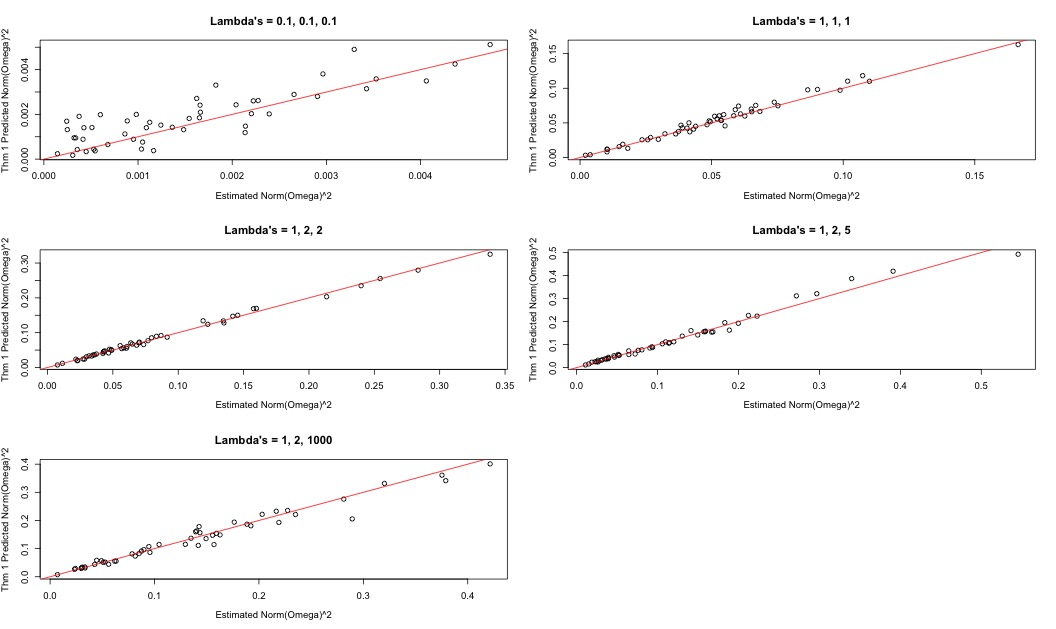
\includegraphics[scale=0.4]{UnderestimatingOmega_Multipliers_Theorem.jpeg}\\
(The above data were simulated assuming $\tilde{\bm{\Xi}} \sim MN_{3 \times 100}\left( \bm{0}, I_3, I_{100} \right)$, $\bm{E} \sim MN_{p \times 100}\left( \bm{0}, \text{diag}\left( 0.15, \ldots, 0.15 \right), I_{100} \right)$. The elements of $\tilde{\bm{L}}$ are independent normals with variance chosen to get the correct $\mathcal{I}_{\text{confounding}} = \text{diag}\left( \frac{\lambda_1}{100}, \frac{\lambda_2}{100}, \frac{\lambda_3}{100} \right)$)

\indent We can illustrate the effect of the size of $\mathcal{I}_{\text{confounding}}$ on the extent of the shrinkage in $\hat{\tilde{\bm{\Omega}}}$ with a simple simulation. We first fix the effect due to cell type, $\tilde{\bm{L}}$, and the residual variability, $\bm{\Sigma}$, s.t. $\frac{1}{p}\tilde{\bm{L}}^T \bm{\Sigma}^{-1}\tilde{\bm{L}} = \frac{\lambda}{n}I_K$. We also fix a $2 \times n$ design matrix $\bm{X} = \left[ \begin{matrix}
\text{Intercept}\\
\text{Disease Status (0's and 1's)}
\end{matrix} \right]$. We then simulate data according to \textbf{Equ. 11} by varying the observed correlation between cell type and covariate of interest ($\tilde{\bm{\Omega}}^{(\text{OLS})}$) and see how significantly $\hat{\tilde{\bm{\Omega}}}$ underestimates the observed correlation. Below are our results:\\
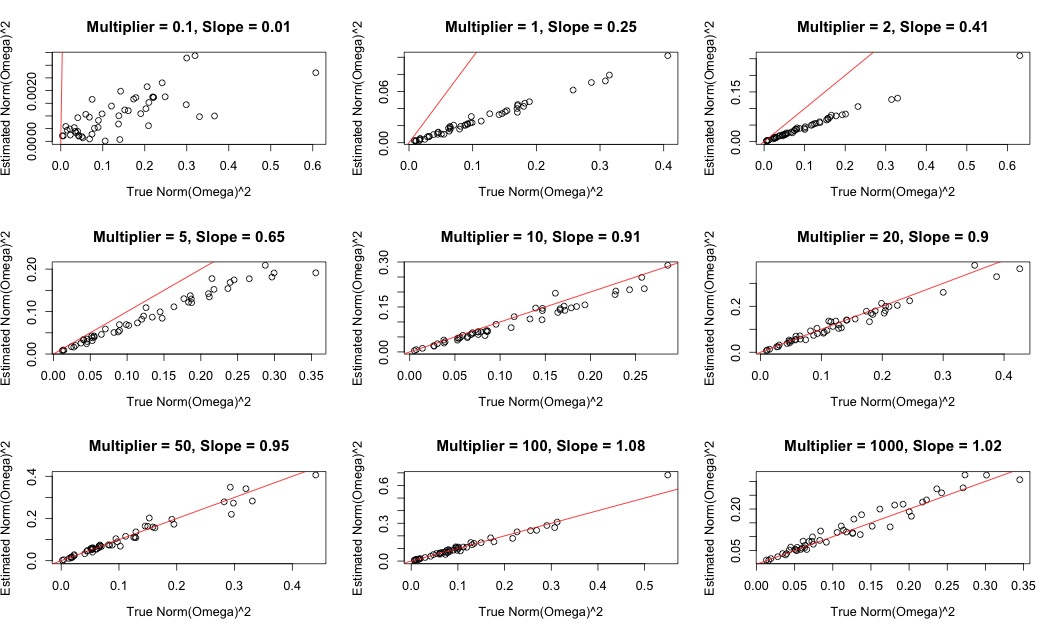
\includegraphics[scale=0.4]{UnderestimatingOmega_Multipliers.jpeg}\\
\\
It is clear that the less informative the methylation data are for cell type (i.e. the smaller $\frac{1}{p}\tilde{\bm{L}}^T \bm{\Sigma}^{-1}\tilde{\bm{L}}$ is), the more difficult it is to estimate the observed correlation between cell type and the covariate(s) interest.\\
\indent Based on the above results, we can identify realistic scenarios when it will be difficult to estimate the correlation between cell type and the covariate(s) of interest. The first is when the non-standardized cell type effect $\bm{L}$ is small, causing only subtle differences in methylation between cell types. This can occur when cells are taken from the same tissue with little observable cellular heterogeneity. Another related possibility is that the majority of CpG sites have the same methylation status across cell types and only a few CpG's have different methylation patterns across cells. If the cell type effects for only a few of the CpG sites are large, then underestimating the variance given by\textbf{equ. 11} can have serious repercussions on the accuracy of any false discovery procedure (need to add an FDR plot). A third may occur when the covariate(s) of interest explains the majority of the variability in cellular heterogeneity. For example, if our covariate of interest is asthma status and everyone with asthma has one cell type composition and everyone without asthma has a different cell type composition, then there is no way to distinguish the cell type effect from the asthma effect and it is impossible to estimate $\tilde{\bm{L}}$, regardless of the sample size. Mathematically speaking, this occurs when the residual variance $\bm{\Lambda}$ from $\bm{3}$ and $\bm{4}$ is small, meaning $\bm{\tilde{L}} = \bm{L}\bm{\Lambda}^{1/2}$ is small.

\section{Real Data Example}
Our motivating example came from whole-blood methylation data collected from individuals in the Amish and Hutterite communities, two founder populations with little genetic diversity. The goal of this experiment was to study any potential differences in the two population's methylome. We quantified the methylation from $p = 327,273$ CpG sites from 30 Amish and 30 Hutterite adolescents (ages 7-14) using 450K Illumina chips and measured the whole-blood cell composition for 29 of the Amish and all 30 of the Hutterite adolescents using flow cytometry. The design matrix for this experiment was
\begin{equation}
\bm{X} = \left[ \begin{matrix}
\text{Intercept}\\
\text{Amish (1) or Hutterite (0)}
\end{matrix}\right]
\end{equation}
and the cell type composition matrix was
\begin{equation}
\bm{C} = \left[ \begin{matrix}
\text{\begin{turn}{90}
Tcells
\end{turn}} &
\text{\begin{turn}{90}
Bcells
\end{turn}} &
\text{\begin{turn}{90}
Eosinophils
\end{turn}} &
\text{\begin{turn}{90}
Neutroophils
\end{turn}} &
\text{\begin{turn}{90}
Monocytes
\end{turn}}
\end{matrix} \right].
\end{equation}
\\
\indent Since we have access to whole-blood cell composition for 59 of the 60 study subjects, we have the luxury of comparing inference on $\bm{B}$ when cell type is and is not observed (we only use the $n=59$ subjects with observed cell type to compare inference). When we assumed cell type was observed, we modeled the data as
\begin{equation}
\bm{Y}_{p \times n} = \bm{B}_{p \times d}\bm{X}_{d \times n} + \bm{L}_{p \times K}\bm{C}_{K \times n} + \bm{\Gamma}_{p \times r}\bm{V}_{r \times n} + \bm{E}_{p \times n}
\end{equation}
\begin{equation}
\bm{B} = \left[ \begin{matrix}
\mu_1 & b_{(A-H)_1}\\
\vdots & \vdots\\
\mu_p & b_{(A-H)_p}
\end{matrix} \right]
\end{equation}
where the term $\bm{\Gamma}_{p \times r}\bm{V}_{r \times n}$ was included to take into account the effect of unmeasured covariates $\bm{V}$ and $\mu_i$ and $b_{(A-H)_i}$ are the global mean and Amish-Hutterite contrast at CpG $i$. We further assumed that $\bm{V} \sim MN_{r \times n}\left( \bm{\alpha}_{r \times d}\bm{X}_{d \times n}, I_r, I_n \right)$. For simplicity we set $\bm{\alpha} = \bm{0}$, although the inference we did on $\bm{B}$ would not change if we assumed $\bm{\alpha} \neq \bm{0}$ because we needed to account for any spurious correlation between the unmeasured covariates $\bm{V}$ and $\bm{X}$. In order to correct for cell type heterogeneity in this scenario, we simply regressed out $\bm{C}$, meaning the cell type-corrected model was
\begin{equation}
\bm{Y}^{(c)} = \bm{B}\bm{X}^{(c)} + \bm{\Gamma}\bm{V}^{(c)} + \bm{E}^{(c)}
\end{equation}
\begin{equation}
\bm{Y}^{(c)} = \bm{Y}P_{\bm{C}^T}^{\perp}, \quad \bm{V}^{(c)} = \bm{V}P_{\bm{C}^T}^{\perp}, \quad \bm{E}^{(c)} = \bm{E}P_{\bm{C}^T}^{\perp}
\end{equation}
We estimated $r=4$ additional unobserved factors using BCV (cite Wang, Hastie paper) and used CATE to compute any spurious correlation between $\bm{V}^{(c)}$ and $\bm{X}^{(c)}$, as well as $\hat{\bm{B}} = \left[ \begin{matrix}
\hat{\mu}_1^{(\text{cell})} & \hat{b}_{(A-H)_1}^{(\text{cell})}\\
\vdots & \vdots\\
\hat{\mu}_p^{(\text{cell})} & \hat{b}_{(A-H)_p}^{(\text{cell})}
\end{matrix} \right]$. Our test statistic used to infer the difference in methylation at CpG site $i$ between Amish and Hutterite adolescents was then
\begin{equation}
\hat{t}_i^{(\text{cell})} = \frac{\hat{b}_{(A-H)_i}^{(\text{cell})}}{\sqrt{\hat{\text{Var}}\left( \hat{b}_{(A-H)_i}^{(\text{cell})} \right)}}
\end{equation}
where $\hat{\text{Var}}\left(\hat{b}_{(A-H)_1}^{(\text{cell})} \right)$ was computed according to \textbf{equ. 11}. We used a $t$-distribution with $n - K - d - r = 48$ degrees of freedom to compute p-values at each CpG site $i = 1, \ldots, p$ to test for differential methylation.\\ 
\indent When cell type is UNOBSERVED, we combined unmeasured covariates $\bm{C}$ and $\bm{V}$ in \textbf{equ. 22} and modeled the data as
\begin{equation}
\bm{Y}_{p \times n} = \bm{B}_{p \times d}\bm{X}_{d \times n} + \tilde{\bm{L}}_{p \times K'}\tilde{\bm{\Omega}}_{K' \times d}\bm{X}_{d \times n} + \tilde{\bm{L}}_{p \times K'}\tilde{\bm{\Xi}}_{K' \times n} + \bm{E}_{p \times n}
\end{equation}
where $\tilde{\bm{\Omega}} = \left[ \begin{matrix}
\bm{\Lambda}^{-1/2}\bm{\Omega}\\
\bm{\alpha}
\end{matrix} \right]$, $\bm{\tilde{L}} = \left[ \begin{matrix}
\bm{L}\Lambda^{1/2} & \bm{\Gamma}
\end{matrix} \right]$ and $\tilde{\bm{\Xi}} = \left[ \begin{matrix}
\Lambda^{-1/2}\bm{\Xi}\\
\bm{V}
\end{matrix} \right]$. We used the exact same procedure as above to estimate $K' = 6$, $\hat{\tilde{\bm{\Omega}}}$ and $\hat{\bm{B}} = \left[ \begin{matrix}
\hat{\mu}_1^{(\text{no cell})} & \hat{b}_{(A-H)_1}^{(\text{no cell})}\\
\vdots & \vdots\\
\hat{\mu}_p^{(\text{no cell})} & \hat{b}_{(A-H)_p}^{(\text{no cell})}
\end{matrix} \right]$. And just as we did when we observed each individual's whole-blood cell composition, we let
\begin{equation}
\hat{t}_i^{(\text{no cell})} = \frac{\hat{b}_{(A-H)_i}^{(\text{no cell})}}{\sqrt{\hat{\text{Var}}\left( \hat{b}_{(A-H)_i}^{(\text{no cell})} \right)}}
\end{equation}
and computed p-values to test for differential methylation between both groups using a $t$-distribution with $n - d - K' = 51$ degrees of freedom. Below are p-value histrograms that compare our results when we assume cell composition are and are not observed:\\
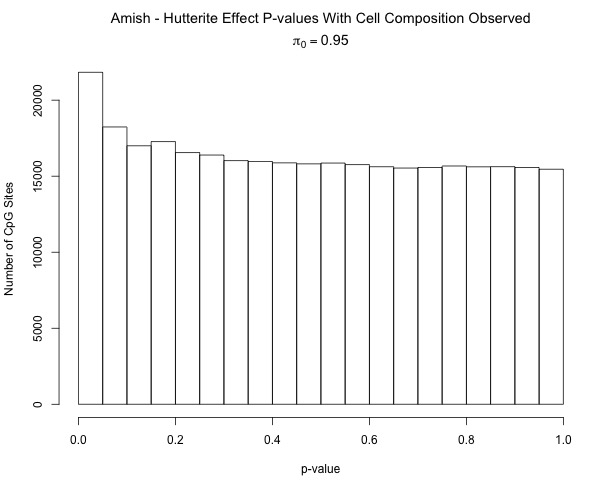
\includegraphics[scale=0.4]{AmishHutterite_CellPvalues.jpeg}
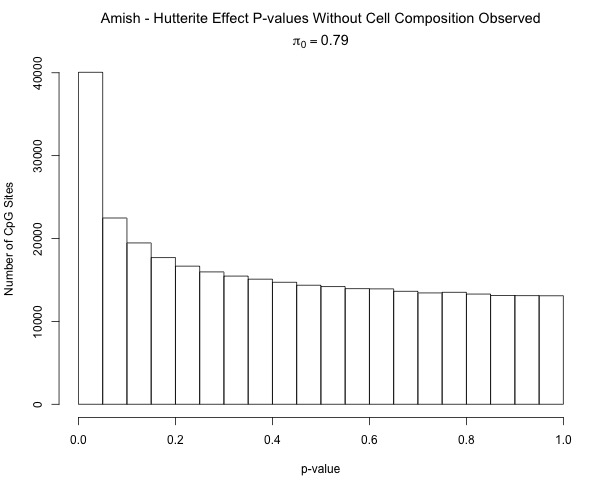
\includegraphics[scale=0.4]{AmishHutterite_noCellPvalues.jpeg}\\
\indent The stark difference between these results is because of the correlation between whole-blood cell composition and group status. The table below gives the standardized regression coefficients after regressing cell type $\bm{C}$ onto Amish vs. Hutterite group status $\bm{X}$:\\
\\
\begin{tabular}{ |p{1.5cm}||p{3cm}| }
\hline
Cell Type & Amish $-$ Hutterite Standardized Effect\\
\hline
T cell & $-0.62$\\\hline
B cell & $0.65$\\\hline
Eosinophil & $-0.40$\\\hline
Neutrophil & $1.41$\\\hline
Monocyte & $0.65$\\\hline
\end{tabular}\\

Since cell heterogeneity and group status are so correlated, there is little variability left in $\bm{X}$ to estimate $\bm{B}$ after we correct for cell type (i.e. we are in the scenario when $\bm{\Lambda}^{1/2}$ is small), which in turn cause our test statistics to move closer to 0. We also estimated $\tilde{\bm{L}}$ and found that $\left( \frac{\abs{\frac{1}{p}\hat{\tilde{\bm{L}}}^T \hat{\bm{\Sigma}}^{-1}\hat{\tilde{\bm{L}}}}}{\abs{\frac{1}{59} I_5}} \right)^{1/5} \approx 1.3$. This implies that if $\tilde{\bm{L}}$ is non-zero and cellular heterogeneity were not observed, the observed CpG methylation data would not be informative enough to estimate cell type and we would perform considerable anti-conservative inference. However, just because $\abs{\frac{1}{p}\hat{\tilde{\bm{L}}}^T \hat{\bm{\Sigma}}^{-1}\hat{\tilde{\bm{L}}}}$ is slightly larger than $\abs{\frac{1}{59} I_5}$ does not mean the inference we do without measured cell type is anti-convervative. In fact, if $\tilde{\bm{L}} = \bm{0}$, we would expect $\frac{1}{p}\hat{\tilde{\bm{L}}}^T \hat{\bm{\Sigma}}^{-1}\hat{\tilde{\bm{L}}} \approx \frac{1}{59} I_5$. Therefore, we cannot say with 100\% confidence that the results without cell type measurements are anti-conservative. We can only use our prior understanding of methylation patterns across different cell types and assume that $\tilde{\bm{L}} \neq \bm{0}$. If this were in fact the case, our sample size is not large enough to perform accurate inference without having observed cell composition.

\section{Simulation Study}
\indent Incorrectly estimating the correlation between cell type heterogeneity and the covariate(s) of interest can have deleterious effects on any procedure that attempts to control for false discovery. To explore this, we simulated data according to \textbf{equ. 5} with parameters based on estimates in the Amish-Hutterite study (see below table). We partitioned $n = 100$ individuals into two groups, 50 of them Amish and 50 of them Hutterites. In all of our simulations, methylation differed in only one cell type, i.e. $K=1$.\\
\\
\begin{tabular}{|p{2.0cm}||p{3.1cm}|p{2.8cm}|p{2.0cm}|p{3.5cm}|}
\hline
Simulation ID & Amish-Hutterite Stand. Effect, $B$ & Cell Type Stand. Effect, $L$ & $\mathcal{I}_{\text{condounding}} = \frac{1}{p}L^T \Sigma^{-1}L$ & Observed Correlation btwn. $\bm{X}$ and $\bm{C}$, $\tilde{\bm{\Omega}}^{\text{OLS}}$\\\hline
(a) & $0.95\delta_0 + 0.05N\left( 0,0.4 \right)$ & $0.7\delta_0 + 0.3N\left( 0, \tau_1 \right)$ & $\frac{1.3}{n}I_1$ & 1.41\\\hline
(b) & $0.95\delta_0 + 0.05N\left( 0,0.4 \right)$ & $0.7\delta_0 + 0.3N\left( 0, \tau_3 \right)$ & $\frac{1.3 \times 10}{n}I_1$ & 1.41 \\\hline
(c) & $0.95\delta_0 + 0.05N\left( 0,0.4 \right)$ & $0.7\delta_0 + 0.3N\left( 0, \tau_2 \right)$ & $\frac{1.3}{10n}I_1$ & 1.41 \\\hline
(d) & $0.95\delta_0 + 0.05N\left( 0,0.4 \right)$ & $0.7\delta_0 + 0.3N\left( 0, \tau_4 \right)$ & $\frac{1.3}{n}I_1$ & $1.41/3$\\\hline

\end{tabular}\\
The above table gives the parameters for the four different simulations, where the variances $\tau_i$ were chosen to get the correct $\mathcal{I}_{\text{confounding}}$. The below figures plot Storey's q-value against the true false discovery proportion
\begin{equation}
FDP(q) = \frac{\#\left\lbrace \text{False positives with q-values $\leq q$} \right\rbrace}{\#\left\lbrace \text{CpG sites with q-values $\leq q$} \right\rbrace}
\end{equation}
\\
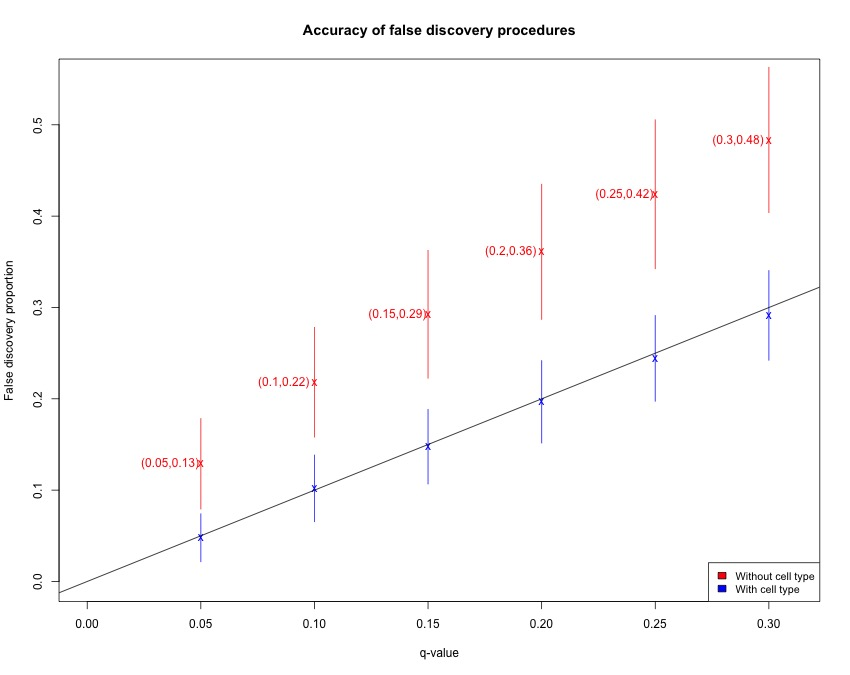
\includegraphics[scale=0.25]{Fdp_1p3_pi00p7.jpeg}(a)
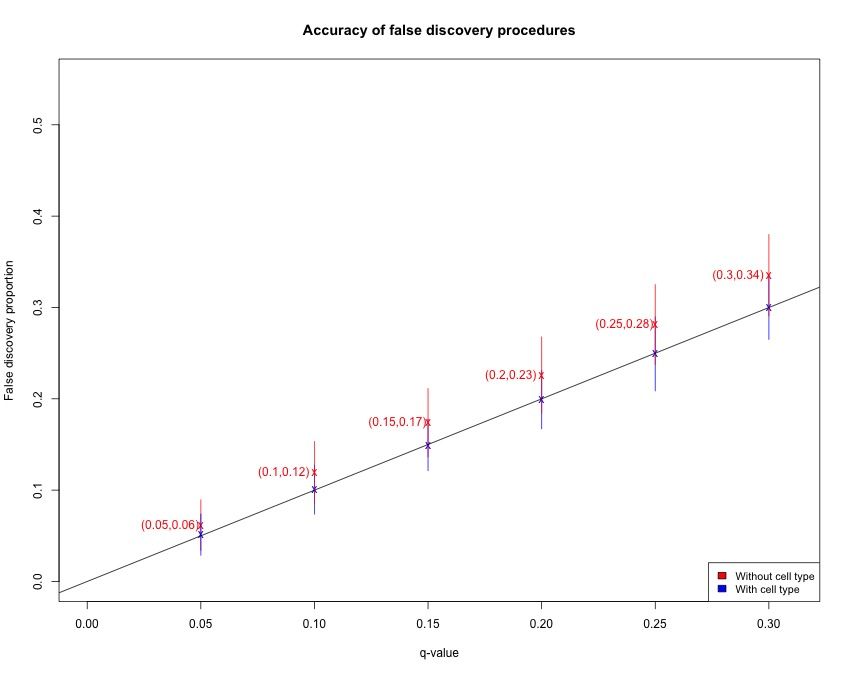
\includegraphics[scale=0.25]{Fdp_13p0.jpeg}(b)\\
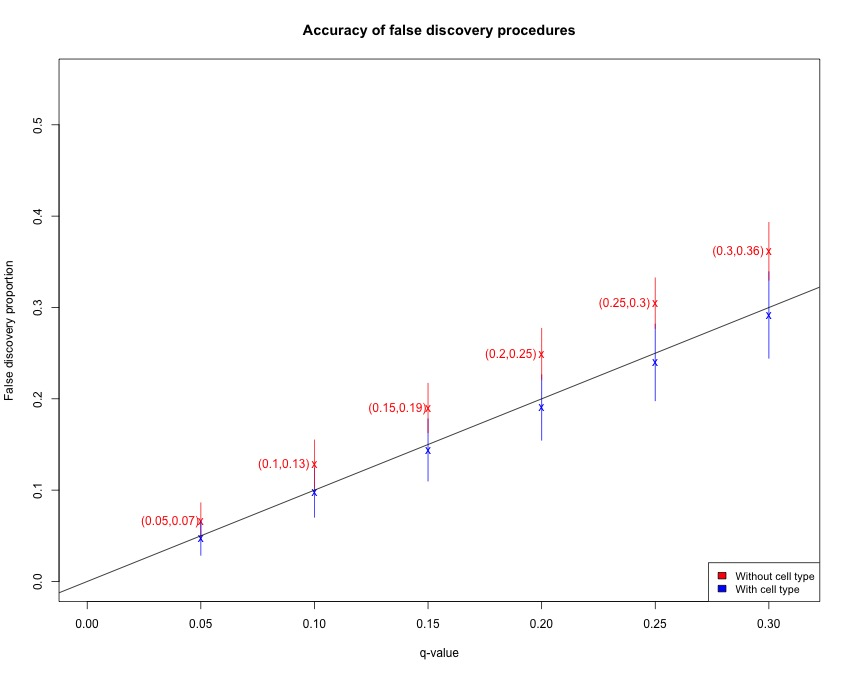
\includegraphics[scale=0.25]{Fdp_0p13.jpeg}(c)
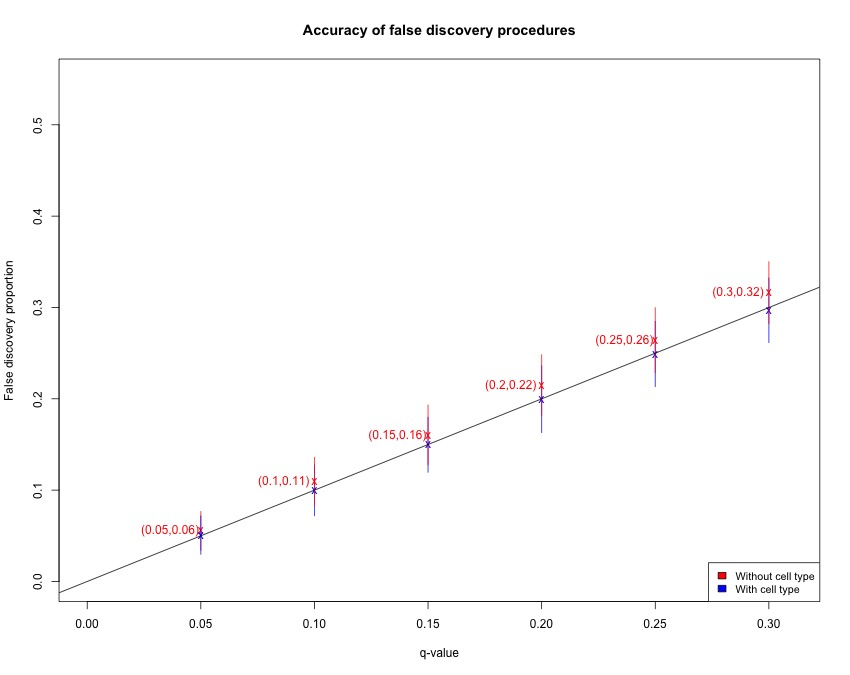
\includegraphics[scale=0.25]{Fdp_1p3p0_0p33xcorr.jpeg}(d)\\
\\
It is not hard to see that when the correlation $\tilde{\bm{\Omega}}^{\text{OLS}}$ is large and we have little power to estimate it (plot (a)), we incur significantly more false positives than we would expect using a reasonable false discovery control procedure. The reason for this is two fold. First, when we underestimate $\tilde{\bm{\Omega}}^{\text{OLS}}$ our estimator for $\hat{B}$ is significantly biased and second, we will underestimate the variance of the components of $\hat{B}$ (see \textbf{equ. 9}). However, is we have enough statistical power to accurately estimate $\tilde{\bm{\Omega}}^{\text{OLS}}$ (plot (b)), our false discovery control procedure is accurate. We also note that if the cell type effect is very small in comparison to the effect of interest (simulation (c)), we significantly underestimate $\tilde{\bm{\Omega}}^{\text{OLS}}$ but still can accurately control false discovery. This is because the effect $\tilde{\bm{L}}\tilde{\bm{\Omega}}^{\text{OLS}} \bm{X}$ is much smaller in comparison to $\bm{B}\bm{X}$, so we tend to find true non-zero Amish-Hutterite effects before Amish-Hutterite effects that are just due to differences in cell composition. Similar reasoning explains why we can control for false discovery when $\tilde{\bm{\Omega}}^{\text{OLS}}$ is small (as in simulation (d)). Even though we underestimate $\tilde{\bm{\Omega}}^{\text{OLS}}$, $\tilde{\bm{\Omega}}^{\text{OLS}} - \hat{\tilde{\bm{\Omega}}}$ is innocuously small.

\section{Partially Observed Cell Type}
\indent So far we have explored methods to correct for cell type with $\bm{C}$ measured and not measured. When $\bm{C}$ is measured, estimation reduces to ordinary least squares for which the statistical properties are well understood. When $\bm{C}$ is not measured, we showed that correcting for cell type becomes challenging when the methylation data are not informative for cell composition. Specifically, we showed that we tend to underestimate the correlation between cell type and the covariate of interest, $\tilde{\bm{\Omega}}^{(OLS)}$, when the average size of the cell type effect is on the order or less than the statistical error, $\frac{1}{\sqrt{n}}$. The remaining unexplored regime is when we measure cell type composition for only a fraction of the $n$ individuals. In this section we consider this scenario to determine if/when we can accurately correct for cell type heterogeneity without having to measure it on all $n$ individuals.\\
\indent Suppose we have measured cell type composition for $n_1$ out of the $n$ individuals and do not observe the cell composition for the other $n_2 = n - n_1$ individuals. We can split the data into two groups: those with cell type observed and those without cell type observed:
\begin{equation}
\bm{Y}_1 = \bm{B}\bm{X}_1 + \bm{L}\bm{C}_1 + \bm{E}_1
\end{equation}
and
\begin{equation}
\bm{Y}_2 = \bm{B}\bm{X}_2 + \bm{L}\bm{C}_2 + \bm{E}_2
\end{equation}
where we observe $\bm{X}_1, \bm{X}_2$ and $\bm{C}_1$, but not $\bm{C}_2$. We also make the same assumptions on the residual matrices $\bm{E}_i$, i.e. $\bm{E}_i \sim MN_{p \times n_i}\left( \bm{0}, \bm{\Sigma}=\text{diag}\left( \sigma_1^2, \ldots, \sigma_p^2 \right), I_{n_i} \right)$. Lastly, we assume that the covariates $\bm{X}$ and cell types $\bm{C}$ are sampled in a way such that
\begin{equation}
\lim_{n \to \infty} \bm{C}\bm{X}^T \left( \bm{X}\bm{X}^T \right)^{-1} \to \bm{\Omega} \in \mathbb{R}^{K \times d}
\end{equation}
\begin{equation}
\lim_{n_i \to \infty}\frac{1}{n_i-d} \bm{C}_i P_{\bm{X}_i^T}^{\perp}\bm{C}_i^T \to \bm{\Lambda} \succ \bm{0} \in \mathbb{R}^{K \times K}.
\end{equation}
After we rotate $\bm{Y}_i$ by an orthonormal basis for the kernel of $\bm{X}_i$ in \textbf{(94)} and \textbf{(95)}, we get
\begin{equation}
\bm{Y}_1\bm{Q}_1 =  \tilde{\bm{Y}}_1 = \bm{L}\tilde{\bm{C}}_1 + \tilde{\bm{E}}_1
\end{equation}
and
\begin{equation}
\bm{Y}_2\bm{Q}_2 = \tilde{\bm{Y}}_2 = \bm{L}\tilde{\bm{C}}_2 + \tilde{\bm{E}}_2
\end{equation}
where $\bm{Q}_i \bm{Q}_i^T = P_{\bm{X}_i^T}^{\perp}$ and $\tilde{\bm{E}}_i \sim MN_{p \times \left( n_i - d \right)} \left( \bm{0}, \bm{\Sigma}, I_{n_i - d} \right)$. Our goal is to determine the conditions on $n_1$, $n_2$, $p$ and $\bm{L}$ under which we can perform reliable inference on $\bm{B}$.\\
\indent If $\hat{\bm{L}}$ was an estimate for $\bm{L}$, then our estimate for $\bm{B}$ would be
\begin{equation}
\hat{\bm{B}} = \left[ \begin{matrix}
\bm{Y}_1 - \hat{\bm{L}}\bm{C}_1 & \bm{Y}_2 - \hat{\bm{L}}\hat{\bm{\Omega}}_1\bm{X}_2
\end{matrix} \right]\left[ \begin{matrix}
\bm{X}_1 & \bm{X}_2
\end{matrix} \right]^T \left( \left[ \begin{matrix}
\bm{X}_1 & \bm{X}_2
\end{matrix} \right] \left[ \begin{matrix}
\bm{X}_1 & \bm{X}_2
\end{matrix} \right]^T \right)^{-1}
\end{equation}
where $\hat{\bm{\Omega}}_1 = \bm{C}_1\bm{X}_1^T \left( \bm{X}_1\bm{X}_1^T \right)^{-1}$. Note that unlike the GLS estimator, the estimate $\hat{\bm{\Omega}}_1$ is consistent when the data $\bm{Y}$ are not informative for cell type. Therefore, in order to do accurate inference on $\bm{B}$, we must first have an accurate estimator for $\bm{L}$. If we were to just use the first set of individuals to estimate $\bm{L}$, standard OLS will give us an estimator $\hat{\bm{L}}_{\text{OLS}_1} = \left[ \begin{matrix}
\bm{\ell}_{1,{\text{OLS}_1}}^T \\
\vdots\\
\bm{\ell}_{p,{\text{OLS}_1}}^T
\end{matrix} \right]$ with $\bm{\ell}_{g,{\text{OLS}_1}} = \bm{\ell}_g + \mathcal{O}_P\left( \frac{1}{\sqrt{n_1}} \right)$. It stands to reason, however, that we could potentially get a better estimator for $\bm{L}$ by incorporating the covariance information of $\tilde{\bm{Y}}_2$ (unconditional on $\bm{C}_2$), which is a function of $\bm{L}$. To do so, we use the first set of samples to define the empirical cell type covariance matrix $\hat{\bm{\Lambda}}_1 = \frac{1}{n_1-d} \tilde{\bm{C}}_1 \tilde{\bm{C}}_1^T = \frac{1}{n_1-d} \bm{C}_1 P_{\bm{X}_1^T}^{\perp}\bm{C}_1^T$ and study the likelihood function
\begin{equation}
\ell\left( \bar{\bm{L}}, \bm{\Sigma}, \bm{W} \right) = \alpha_1 \ell_1\left( \bar{\bm{L}}, \bm{\Sigma} \right) + \alpha_2 \ell_2\left( \bar{\bm{L}}, \bm{\Sigma}, \bm{W} \right)
\end{equation}
\begin{equation}
\ell_1\left( \bar{\bm{L}}, \bm{\Sigma} \right) = -\frac{1}{p}\log\abs{\bm{\Sigma}} - \frac{1}{n_1 p}\Tr\left[ \left( \tilde{\bm{Y}}_1 - \bar{\bm{L}}\tilde{\bm{C}}_1 \right)^T \bm{\Sigma}^{-1}\left( \tilde{\bm{Y}}_1 - \bar{\bm{L}}\tilde{\bm{C}}_1 \right) \right]
\end{equation}
\begin{equation}
\ell_2\left( \bar{\bm{L}}, \bm{\Sigma}, \bm{W} \right) = -\frac{1}{p}\log\abs{\bm{\Sigma}} - \frac{1}{n_2 p}\Tr\left[ \left( \tilde{\bm{Y}}_2 - \bar{\bm{L}}\bm{W} \right)^T \bm{\Sigma}^{-1}\left( \tilde{\bm{Y}}_2 - \bar{\bm{L}}\bm{W} \right) \right], \quad \frac{1}{n_2}\bm{W}\bm{W}^T = \hat{\bm{\Lambda}}_1
\end{equation}
where $\alpha_i = \frac{n_i}{n}$. Suppose first that $\alpha_1 = 0$ and $\bm{\Sigma}, \bm{\Lambda}$ were known. Then $\ell\left( \bm{L}, \bm{\Sigma}, \bm{W} \right)$ is maximized by scaled versions of the first $K$ left and right singular values of the matrix $\frac{1}{\sqrt{n_2}}\Sigma^{-1}\bm{Y}_2$. However, from the work we did above, we know that the limit of $\frac{n}{p}\bm{L}^T \bm{\Sigma}^{-1}\bm{L}$ must be positive definite for us to be able to correctly pick out the the loadings corresponding to the $K$ columns of $\bm{L}$. If not, our estimate will just be noise. Therefore, we intuitively expect that the limit of $\frac{n}{p}\bm{L}^T \bm{\Sigma}^{-1}\bm{L}$ must be positive definite for us to be able to use the second set of individuals to reduce the variability in our estimate for $\bm{L}$. 

 We immediately see that if $\alpha_1 \to 0$, then we are not guaranteed that \textbf{(100)} will give us an unbiased estimator. For example, if $\bm{\Lambda} = I_K$ and $\alpha_1 = 0$, then our estimate for $\bm{L}$ will only be unique up to rotation. However, this rotation matrix will not be incorporated into the estimate $\hat{\bm{\Omega}}_1$, meaning $\hat{\bm{L}}\hat{\bm{\Omega}}_1$ will be a severely biased estimate for $\bm{L}\bm{\Omega}^{(\text{OLS})}$. We therefore assume that $\frac{n_1}{n_2} \to c > 0$.

\section{What I need to add}
\begin{itemize}
\item My model with partially observed cell type. I only have simulation results here. I should include a brief discussion about the caveats with real data, since additional batch effects may be difficult to estimate.
\item A discussion when the residual $E$ is not normally distributed. The confidence we have in factor analysis will depend on the higher order cumulants (notably the fourth kumulant) when the residuals are not normally distributed. This is important when we attempt to diagnose datasets with confounding we cannot estimate (i.e. how much does $\frac{1}{p}\hat{\Gamma}^T\hat{\Sigma}^{-1}\hat{\Gamma}$ differ from $\frac{1}{p}\Gamma^T \Sigma^{-1}\Gamma$ as a function of the distribution of $E$).
\end{itemize}

\section{Partially Observed Data Notes}
Let $\hat{L}$ and $\hat{L}_{OLS}$ be the partially observed and OLS estimates for $L$. Define $J = \Sigma + LL^T$, $M_i = \frac{1}{n_i}C_iC_i^T$ and $M = \frac{1}{n}CC^T$. We assume throughout that $M_1 = I_K$. Some observations from simulation are:
\begin{itemize}
\item As $n,p,\frac{p}{n} \to \infty$, $\hat{L}_{OLS}$ and $\hat{L}$ seem to be close. That is, it appears that under the correct asymptotic regime $\sqrt{n}\norm{\hat{\ell}_{OLS_g} - \hat{\ell}_g} \to 0$. If I can prove this, the problem is finished.
\item If we let $\hat{M}_{OLS_2} = I_K - \hat{L}_{OLS}\hat{J}_{OLS}^{-1}\hat{L}_{OLS} + \hat{L}_{OLS}^T \hat{J}_{OLS}^{-1} S_2\hat{J}^{-1}_{OLS}\hat{L}_{OLS}$, then it appears that under the right conditions on $n,p$, $\sqrt{n}\norm{\hat{M}_{OLS_2} - M_2} \to 0$. What's even more amazing is that if we let $\hat{M}_2 = I_K - \hat{L}^T\hat{J}^{-1}\hat{L} + \hat{L}^T \hat{J}^{-1} S_2\hat{J}^{-1}\hat{L}$, then $\frac{\norm{\hat{M}_{2} - M_2}}{\norm{\hat{M}_{OLS_2} - M_2}} \to f\left( \alpha_2 \right)$. The values of $f$ I have observed have been
	\begin{itemize}
	\item $f\left( 1/4 \right) \approx 2$	
	\item $f\left( 1/2 \right) \approx 3$
	\item $f\left( 1 \right) = \infty$
	\item $f\left( 0 \right) = 1$
	\end{itemize}
Note that if I can prove this, then the proof is complete. Further, if we can find $f$ then we can also describe how $\alpha_2$ affects the fidelity of our estimator.\\
\\

\end{itemize}
 Some results that we may need are:
\begin{equation}
\frac{n}{p}\hat{L}_{OLS}^T \Sigma^{-1}\hat{L}_{OLS} = \frac{n}{p}\bar{L}^T \Sigma^{-1}\bar{L} + M^{-1} + \mathcal{O}_p\left( \frac{1}{\sqrt{p}} \right)
\end{equation}
\begin{equation}
\frac{n}{p}\hat{L}_{OLS}^T \Sigma^{-1}\bar{L} = \frac{n}{p}\bar{L}^T \Sigma^{-1}\bar{L} + \mathcal{O}_P\left( \frac{1}{\sqrt{p}} \right)
\end{equation}
\begin{equation}
I_K - L^T J^{-1}L = I_K - \left( I_K + L^T\Sigma^{-1}L \right)^{-1}L^T\Sigma^{-1}L = \left( I_K + L^T\Sigma^{-1}L \right)^{-1}
\end{equation}
\begin{equation}
Y^T J^{-1} L = Y^T\Sigma^{-1}L - Y^T\Sigma^{-1}L\left( I_K + L^T\Sigma^{-1}L \right)^{-1} L^T\Sigma^{-1}L = Y^T\Sigma^{-1}L \left( I_K + L^T\Sigma^{-1}L \right)^{-1}
\end{equation}
The score equations for the quasi likelihood will be satisfied $\Leftrightarrow$ we can find an estimator $L = \hat{L}$ s.t.
\begin{multline}
L = \left[ \alpha_1 \frac{1}{n_1}Y_1 C_1^T + \alpha_2 \frac{1}{n_2}Y_2 Y_2^T J^{-1}L \right] \left[ \alpha_1 \underbrace{\frac{1}{n_1}C_1C_1^T}_{I_K} + \alpha_2\left( I_K - L^T J^{-1}L + L^T J^{-1}S_2 J^{-1}L \right) \right]^{-1}=\\
\left[ \alpha_1 \frac{1}{n_1}Y_1 C_1^T + \alpha_2 \frac{1}{n_2}Y_2 Y_2^T J^{-1}L \right] \left[ \alpha_1 I_K + \alpha_2\left( \left( I_K + L^T\Sigma^{-1}L \right)^{-1} + \left( I_K + L^T\Sigma^{-1}L \right)^{-1} L^T\Sigma^{-1}S_2\Sigma^{-1}L \left( I_K + L^T\Sigma^{-1}L \right)^{-1} \right) \right]^{-1}.
\end{multline}
Note that this looks identical to the OLS estimator, when 
\begin{equation}
\hat{C}_2^T = Y_2^T J^{-1}L = Y_2^T\Sigma^{-1}L \left( I_K + L^T\Sigma^{-1}L \right)^{-1}
\end{equation}
and 
\begin{equation}
\hat{M}_2 = \left( I_K + L^T\Sigma^{-1}L \right)^{-1} + \left( I_K + L^T\Sigma^{-1}L \right)^{-1} L^T\Sigma^{-1}S_2\Sigma^{-1}L \left( I_K + L^T\Sigma^{-1}L \right)^{-1}.
\end{equation}
I now will examine the behavior of $\hat{M}_2^{OLS}$, i.e. when $L = \hat{L}^{OLS} = \bar{L} + EC^T \left( CC^T \right)^{-1} = \bar{L} + E_1C_1^T \left( CC^T \right)^{-1} + E_2C_2^T \left( CC^T \right)^{-1} = \bar{L} + \tilde{E}_1 + \tilde{E}_2$. We then have:
\begin{multline}
\hat{M}_2^{OLS} = \underbrace{\left( I_K + L^T\Sigma^{-1}L \right)^{-1}}_{A^{-1}} + A^{-1} L^T\Sigma^{-1}S_2 \Sigma^{-1}LA^{-1} = A^{-1} + \underbrace{A^{-1}L^T\Sigma^{-1}\bar{L}M_2 \bar{L}^T\Sigma^{-1}LA^{-1}}_{1.)} + \underbrace{\frac{1}{n_2} A^{-1}L^T\Sigma^{-1}\bar{L}C_2E_2^T \Sigma^{-1}LA^{-1}}_{2.)}\\
+ \underbrace{\left( \frac{1}{n_2} A^{-1}L^T\Sigma^{-1}\bar{L}C_2E_2^T \Sigma^{-1}LA^{-1} \right)^T}_{3.)} + \underbrace{\frac{1}{n_2}A^{-1}L^T\Sigma^{-1}E_2E_2^T\Sigma^{-1}LA^{-1}}_{4.)}
\end{multline}
Then,
\begin{enumerate}
\item The behavior of this is known.
\item \begin{equation}
A^{-1}L^T\Sigma^{-1}\bar{L} \left( \underbrace{\frac{1}{n_2}\frac{n}{p}C_2E_2^T\Sigma^{-1}\bar{L}}_{a)} + \underbrace{\frac{1}{n_2}\frac{1}{p}C_2E_2^T \Sigma^{-1}E_2C_2^T M^{-1}}_{b)} + \underbrace{\frac{1}{n_2}\frac{1}{p}C_2E_2^T\Sigma^{-1} E_1C_1^T M^{-1}}_{c)} \right)\left( \frac{n}{p}A \right)^{-1}
\end{equation}
	\begin{enumerate}
	\item \begin{equation}
	\frac{1}{n_2}\frac{n}{p}C_2E_2^T\Sigma^{-1}\bar{L} \sim \sqrt{\frac{n}{p}}\sqrt{\frac{1}{n_2}}MN_{K \times K}\left( 0, M_2, \frac{n}{p}\bar{L}^T\Sigma^{-1}\bar{L} \right) \underbrace{=}_{n_2 = \mathcal{O}(n)} \mathcal{O}_P\left( \frac{1}{\sqrt{p}} \right)
	\end{equation}
	\item \begin{equation}
	\frac{1}{n_2}\frac{1}{p}C_2E_2^T \Sigma^{-1}E_2C_2^T M^{-1} \sim \frac{1}{p}MN_{K \times p}\left( 0, M_2, I_p \right) MN_{K \times p}\left( 0, M_2, I_p \right)^T M^{-1} = M_2M^{-1} + \mathcal{O}_P\left( \frac{1}{\sqrt{p}} \right)
	\end{equation}
	\item \begin{equation}
	\frac{1}{n_2}\frac{1}{p}C_2E_2^T\Sigma^{-1} E_1C_1^T M^{-1} \sim	\frac{1}{p}\underbrace{MN_{k \times p}\left( 0, M_2, I_p \right) MN_{K \times p}\left( 0, M_1, I_p \right)^T}_{independent}M^{-1} \underbrace{=}_{n_2 = \mathcal{O}(n)} \mathcal{O}_P\left( \frac{1}{\sqrt{p}} \right)
	\end{equation}
	Therefore, $2.) = A^{-1}L^T\Sigma^{-1}\bar{L} M_2M^{-1}\left( \frac{n}{p}A \right)^{-1} + \mathcal{O}_P\left( \frac{1}{\sqrt{p}} \right)$
	\end{enumerate}
\item $= \left( \frac{n}{p}A \right)^{-1}M^{-1}M_2 \bar{L}^T\Sigma^{-1}LA^{-1} + \mathcal{O}_P\left( \frac{1}{\sqrt{p}} \right)$	
\item \begin{multline}
\frac{1}{n_2}A^{-1}L^T\Sigma^{-1}E_2E_2^T\Sigma^{-1}LA^{-1} = \underbrace{\frac{1}{n_2}A^{-1}\bar{L}^T\Sigma^{-1}E_2E_2^T\Sigma^{-1}\bar{L}A^{-1}}_{a.)} + \underbrace{\frac{1}{n_2}A^{-1}\bar{L}^T\Sigma^{-1}E_2E_2^T\Sigma^{-1} \tilde{E}A^{-1}}_{b.)} + \underbrace{\left( \frac{1}{n_2}A^{-1}\bar{L}^T\Sigma^{-1}E_2E_2^T\Sigma^{-1} \tilde{E}A^{-1} \right)^T}_{c.)}\\
+ \underbrace{\frac{1}{n_2}A^{-1}\tilde{E}^T\Sigma^{-1}E_2E_2^T\Sigma^{-1} \tilde{E}A^{-1}}_{d.)}
\end{multline}
	\begin{enumerate}
	\item \begin{multline}
	\frac{1}{n_2}A^{-1}\bar{L}^T\Sigma^{-1}E_2E_2^T\Sigma^{-1}\bar{L}A^{-1} \sim \left( \frac{n}{p}A \right)^{-1} \frac{n}{n_2}\frac{1}{p} MN_{K \times n_2}\left( 0, \frac{n}{p}\bar{L}^T\Sigma^{-1}\bar{L}, I_{n_2} \right) MN_{K \times n_2}\left( 0, \frac{n}{p}\bar{L}^T\Sigma^{-1}\bar{L}, I_{n_2} \right)^T \left( \frac{n}{p}A \right)^{-1} = \\
	\frac{n}{p}\left( \frac{n}{p}A \right)^{-1} \frac{n}{p}\bar{L}^T\Sigma^{-1}\bar{L} \left( \frac{n}{p}A \right)^{-1} + \mathcal{O}_P\left( \frac{1}{\sqrt{p}} \right)
	\end{multline}
	
	\item \begin{multline}
	\frac{1}{n_2}A^{-1}\bar{L}^T\Sigma^{-1}E_2E_2^T\Sigma^{-1} \tilde{E}A^{-1} = \underbrace{\frac{1}{n_2p}\left( \frac{n}{p}A \right)^{-1}\bar{L}^T\Sigma^{-1}E_2E_2^T\Sigma^{-1} E_1C_1^T M^{-1}A^{-1}}_{i.)}\\
	+ \underbrace{\frac{1}{n_2p}\left( \frac{n}{p}A \right)^{-1}\bar{L}^T\Sigma^{-1}E_2E_2^T\Sigma^{-1} E_2C_2^T M^{-1}A^{-1}}_{ii.)}
	\end{multline}
		\begin{enumerate}
		\item \begin{equation}
		\frac{1}{n_2p}\left( \frac{n}{p}A \right)^{-1}\bar{L}^T\Sigma^{-1}E_2E_2^T\Sigma^{-1} E_1C_1^T M^{-1}A^{-1} \underbrace{=}_{\Sigma=I_p} \frac{n}{n_2}\frac{1}{\sqrt{p}}\left( \frac{n}{p}A \right)^{-1}\left[ \frac{1}{p}\left( \sqrt{\frac{n}{p}}\bar{L}^T \right) E_2E_2^T E_1 \left( \frac{1}{\sqrt{n}}C_1^T M^{-1} \right)\right]\left( \frac{n}{p}A \right)^{-1}
		\end{equation}
		Let $\sqrt{\frac{n}{p}}\bar{L}^T = R^T Q^T$, where $R = \mathcal{O}_P(1)$ and $Q^T \in \mathbb{R}^{K \times p}$. We can then find a matrix $V$ s.t. $V \in \mathbb{R}^{p \times \left( p-K \right)}$ s.t. $V^TV = I_{p-K}$ and $Q^T V = 0_{K \times \left( p-K \right)}$. We focus on the expression $\frac{1}{p}\left( \sqrt{\frac{n}{p}}\bar{L}^T \right) E_2E_2^T E_1 \left( \frac{1}{\sqrt{n}}C_1^T M^{-1} \right)$.
		\begin{multline}
		\frac{1}{p}\left( \sqrt{\frac{n}{p}}\bar{L}^T \right) E_2E_2^T E_1 \left( \frac{1}{\sqrt{n}}C_1^T M^{-1} \right) = R^T\underbrace{ \frac{1}{p}Q^T E_2 E_2^T Q}_{I_K + \mathcal{O}_P\left( \frac{1}{\sqrt{p}} \right)} \underbrace{Q^T E_1 \left( \frac{1}{\sqrt{n}}C_1^T M^{-1} \right)}_{\mathcal{O}_P(1)} \\
		+ R^T\frac{1}{p} Q^T E_2 E_2^T V V^T E_1 \left( \frac{1}{\sqrt{n}}C_1^T M^{-1} \right)
		\end{multline}	
		$\frac{1}{p} E_2^T V V^T E_1 \left( \frac{1}{\sqrt{n}}C_1^T M^{-1} \right) \in \mathbb{R}^{n \times K}$ is entry-by-entry $\mathcal{O}_P\left( \frac{1}{\sqrt{p}} \right)$. When we hit it with the random matrix $Q^T E_2 \in \mathbb{R}^{K \times n}$ that is independent from everything else, we get a $K \times K$ matrix that is entry-wide $\mathcal{O}_P\left( \sqrt{\frac{n}{p}} \right)$. Therefore, $i.) = \mathcal{O}_P\left( \frac{1}{\sqrt{p}} \right)$.
		
		\item We apply the same strategy for this.
		\begin{equation}
		\frac{1}{n_2p}\left( \frac{n}{p}A \right)^{-1}\bar{L}^T\Sigma^{-1}E_2E_2^T\Sigma^{-1} E_2C_2^T M^{-1}A^{-1} \underbrace{=}_{\Sigma=I_p} \frac{n}{n_2}\frac{1}{\sqrt{p}}\left( \frac{n}{p}A \right)^{-1}\left[ \frac{1}{p}\left( \sqrt{\frac{n}{p}}\bar{L}^T \right) E_2E_2^T E_2 \left( \frac{1}{\sqrt{n}}C_2^T M^{-1} \right)\right]\left( \frac{n}{p}A \right)^{-1}
		\end{equation}
		Then
		\begin{multline}
		\frac{1}{p}\left( \sqrt{\frac{n}{p}}\bar{L}^T \right) E_2E_2^T E_2 \left( \frac{1}{\sqrt{n}}C_2^T M^{-1} \right) = R^T\underbrace{ \frac{1}{p}Q^T E_2 E_2^T Q}_{I_K + \mathcal{O}_P\left( \frac{1}{\sqrt{p}} \right)} \underbrace{Q^T E_2 \left( \frac{1}{\sqrt{n}}C_2^T M^{-1} \right)}_{\mathcal{O}_P(1)} \\
		+ R^T\frac{1}{p} Q^T E_2 E_2^T V V^T E_2 \left( \frac{1}{\sqrt{n}}C_2^T M^{-1} \right)
		\end{multline}
		We see that $\frac{1}{p}E_2^T V V^T E_2 \left( \frac{1}{\sqrt{n}}C_2^T M^{-1} \right)  = \frac{1}{\sqrt{n}}C_2^T M^{-1} + U\Lambda U^T \left(\frac{1}{\sqrt{n}}C_2^T M^{-1}\right)$ where $\Lambda$ is diagonal with entries (almost) bounded between $\left[ -2\sqrt{\frac{n_2}{p}}, +2\sqrt{\frac{n_2}{p}} \right]$ with the asymptotic semicircle distribution. Note that if $\Lambda$ were a multiple of the identity, $Q^T E_2 U\Lambda U^T \left( \frac{1}{\sqrt{n}}C_2^T M^{-1} \right) = \mathcal{O}_P\left( \sqrt{\frac{n_2}{p}} \right)$. The order or magnitude seems to be true in simulation, so I will assume $Q^T E_2 U\Lambda U^T \left( \frac{1}{\sqrt{n}}C_2^T M^{-1} \right) \leq \mathcal{O}_P\left( 1 \right)$. And since $Q^T E_2 C_2^T M^{-1} = \mathcal{O}_P(1)$, $ii.) = \mathcal{O}_P\left( \frac{1}{\sqrt{p}} \right)$.
		\end{enumerate}
	Therefore, $b.) = \mathcal{O}_P\left( \frac{1}{\sqrt{p}} \right)$.
		
	\item This is also $\mathcal{O}_P\left( \frac{1}{\sqrt{p}} \right)$.
	
	\item \begin{multline}
	\frac{1}{n_2}A^{-1}\tilde{E}^T\Sigma^{-1}E_2E_2^T\Sigma^{-1} \tilde{E}A^{-1} = \frac{1}{n_2 p^2} \left( \frac{n}{p}A \right)^{-1} M^{-1}\left[ \underbrace{C_1E_1^T \Sigma^{-1}E_2E_2^T \Sigma^{-1}E_1C_1^T}_{i.)} + \underbrace{C_2E_2^T \Sigma^{-1}E_2E_2^T \Sigma^{-1}E_2C_2^T}_{ii.)}\right]M^{-1}\left( \frac{n}{p}A \right)^{-1} \\
	+ \frac{1}{n_2 p^2}\left( \frac{n}{p}A \right)^{-1} M^{-1}\left[\underbrace{C_2E_2^T \Sigma^{-1}E_2E_2^T \Sigma^{-1}E_1C_1^T}_{iii.)} + \underbrace{\left( C_2E_2^T \Sigma^{-1}E_2E_2^T \Sigma^{-1}E_1C_1^T \right)^T}_{iv.)} \right]M^{-1}\left( \frac{n}{p}A \right)^{-1}
	\end{multline}
		\begin{enumerate}
		\item \begin{equation}
		\frac{1}{n_2 p^2}C_1E_1^T \Sigma^{-1}E_2E_2^T \Sigma^{-1}E_1C_1^T \underbrace{=}_{\tilde{C}_1 = \frac{1}{\sqrt{n_2}} C_1} \left( \frac{1}{p}\tilde{C}_1 E_1^T\Sigma^{-1}E_2 \right) \left( \frac{1}{p}\tilde{C}_1 E_1^T\Sigma^{-1}E_2 \right)^T \underbrace{=}_{simulation} \alpha_1\frac{n}{p}I_K + \underbrace{\mathcal{O}_P\left( \frac{1}{\sqrt{n}} \frac{n}{p} \right)}_{\mathcal{O}_P\left( \frac{1}{\sqrt{p}} \right)}
		\end{equation}
		
		\item Let $P_{C_2^T} = QQ^T$ and $P_{C_2^T}^{\perp} = VV^T$ where $Q \in \mathbb{R}^{n \times K}$ and $V \in \mathbb{R}^{n \times (n-K)}$.
		\begin{multline}
		\frac{1}{n_2 p^2}C_2E_2^T \Sigma^{-1}E_2E_2^T \Sigma^{-1}E_2C_2^T \underbrace{=}_{\tilde{C}_2 = \frac{1}{\sqrt{n_2}} C_2} \frac{1}{p^2}\tilde{C}_2 E_2^T\Sigma^{-1}E_2 E_2^T\Sigma^{-1}E_2 \tilde{C}_2^T \\ = \tilde{R}^T \underbrace{\left( \frac{1}{p} Q^TE_2^T\Sigma^{-1}E_2Q \right)}_{I_K + \mathcal{O}_P\left( \frac{1}{\sqrt{p}} \right)}\underbrace{\left( \frac{1}{p} Q^TE_2^T \Sigma^{-1}E_2Q\right)}_{I_K + \mathcal{O}_P\left( \frac{1}{\sqrt{p}} \right)} \tilde{R} + \underbrace{\frac{1}{p^2}\tilde{R}^T Q^TE_2^T\Sigma^{-1}E_2VV^TE_2^T \Sigma^{-1}E_2Q \tilde{R}}_{\text{same as i.)}}
		\end{multline}
		Therefore, ii.)$ = M_2 + \alpha_2\frac{n}{p}M_2 + \mathcal{O}_P\left( \frac{1}{\sqrt{p}} \right)$
		
		\item \begin{multline}
		\frac{1}{n_2p^2}C_2E_2^T \Sigma^{-1}E_2E_2^T\Sigma^{-1}E_1C_1^T \underbrace{=}_{\frac{1}{\sqrt{n_2}}C_2 = \tilde{C}_2, \frac{1}{\sqrt{n}_2}C_1 = \bar{C}_1} \frac{1}{p^2}\tilde{C}_2 E_2^T \Sigma^{-1}E_2E_2^T\Sigma^{-1}E_1\bar{C}_1^T \underbrace{=}_{\tilde{C}_2^T = Q_2R_2, \bar{C}_1^T = Q_1R_1}\\
		\underbrace{R_2^T}_{\mathcal{O}_P(1)} \underbrace{\left(\frac{1}{p} Q_2^T E_2^T \Sigma^{-1}E_2Q_2 \right)}_{I_K + \mathcal{O}_P\left( \frac{1}{\sqrt{p}} \right)} \underbrace{\left(\frac{1}{p} Q_2^TE_2^T\Sigma^{-1}E_1 Q_1 \right)}_{\mathcal{O}_P\left( \frac{1}{\sqrt{p}} \right)} \underbrace{R_1}_{\mathcal{O}_P(1)} + R_2^T \underbrace{\frac{1}{p^2} Q_2^T E_2^T \Sigma^{-1}E_2V_2 V_2^TE_2^T\Sigma^{-1}E_1 Q_1}_{\mathcal{O}_P\left( \frac{1}{\sqrt{p}}\right) \text{ by simulation}} R_1 = \mathcal{O}_P\left( \frac{1}{\sqrt{p}}\right)
		\end{multline}				
		\item $ = \mathcal{O}_P\left( \frac{1}{\sqrt{p}}\right)$.
		\end{enumerate}
		Therefore, $4d.) = \left( \frac{n}{p}A \right)^{-1} M^{-1}\left[ M_2 + \alpha_1\frac{n}{p}I_K + \alpha_2\frac{n}{p} M_2 \right]M^{-1}\left( \frac{n}{p}A \right)^{-1}$ and
		\begin{equation}
		\text{4.)} = \left( \frac{n}{p}A \right)^{-1}\left[ M^{-1}M_2M^{-1} + \frac{n}{p}\frac{n}{p}\bar{L}^T\Sigma^{-1}\bar{L} + \alpha_1\frac{n}{p}M^{-2} + \alpha_2\frac{n}{p}M^{-1}M_2M^{-1} \right]\left( \frac{n}{p}A \right)^{-1}
		\end{equation}
	\end{enumerate}
\end{enumerate}
Define $\Phi = \frac{n}{p}\bar{L}^T \Sigma^{-1}\bar{L}$ and $A =  \Phi + M^{-1} + \frac{n}{p}I_K$. Then
\begin{multline}
\hat{M}_2^{\text{OLS}} = A^{-1}\left[ \Phi M_2 + \Phi M_2M^{-1} + M^{-1}M_2 \Phi + M^{-1}M_2 M^{-1}\right] A^{-1} + \frac{n}{p}\left[ A^{-1} + \Phi + \alpha_1 M^{-2} + \alpha_2 M^{-1}M_2 M^{-1} \right] + \mathcal{O}_P\left( \frac{1}{\sqrt{p}} \right)\\
= A^{-1}\left( \Phi + M^{-1} \right)M_2 \left( \Phi + M^{-1} \right)A^{-1} + \frac{n}{p}\left[ A^{-1} + \Phi + \alpha_1 M^{-2} + \alpha_2 M^{-1}M_2 M^{-1} \right] + \mathcal{O}_P\left( \frac{1}{\sqrt{p}} \right).
\end{multline}
We see that if the sets of individuals were NOT exchangeable, then $\hat{M}_2^{\text{OLS}} - M_2 = \mathcal{O}_P\left( \sqrt{\frac{n}{p}} \right)$. Therefore, $\hat{M}_2^{\text{OLS}}$ would be a consistent estimator of $M_2$, but it would be $\sqrt{n}$ worse than the $\mathcal{O}_P\left( \frac{1}{\sqrt{p}} \right)$ estimator we want. However, if $M_i - I_K = \mathcal{O}_P\left( \frac{1}{\sqrt{n}} \right)$, then $\frac{n}{p}\left( M_i - I_K \right) = \mathcal{O}_P\left( \frac{1}{\sqrt{p}} \right)$, meaning
\begin{multline}
\frac{n}{p}\left[ A^{-1} + \Phi + \alpha_1 M^{-2} + \alpha_2 M^{-1}M_2 M^{-1} \right] = \frac{n}{p}A^{-1} \left[ \Phi + M^{-1} + \frac{n}{p}I_K + \Phi + \underbrace{\alpha_1 M^{-2} + \alpha_2 M^{-1}M_2 M^{-1}}_{M^{-1}M_2 + \mathcal{O}_P\left( \frac{1}{\sqrt{n}} \right)} \right]A^{-1}\\
= \frac{n}{p}\left[ M_2\Phi + \Phi M_2 + M_2 M^{-1} + M^{-1}M_2 + \frac{n}{p}I_K \right] + \underbrace{\mathcal{O}_P\left( \frac{n}{p}\frac{1}{\sqrt{n}} \right)}_{\leq \mathcal{O}_P\left( \frac{1}{\sqrt{p}} \right) \text{ for $\sqrt{\frac{n}{p}}$ small}}
\end{multline}
Therefore,
\begin{equation}
\hat{M}_2^{\text{OLS}} = A^{-1}\left( \Phi + M^{-1} + \frac{n}{p}I_K \right)M_2 \left( \Phi + M^{-1} + \frac{n}{p}I_K \right)A^{-1} + \mathcal{O}_P\left( \frac{1}{\sqrt{p}} \right) = M_2 + \mathcal{O}_P\left( \frac{1}{\sqrt{p}} \right).
\end{equation}
Now let's look at $\frac{1}{n_2}C_2^T \hat{C}_2$. We see that
\begin{multline}
\frac{1}{n_2}C_2^T \hat{C}_2 = \frac{1}{n_2}C_2^T Y_2^T J^{-1}L = C_2^T Y_2^T \Sigma^{-1}L\left( I_K + L^T\Sigma^{-1}L \right)^{-1} = M_2 \bar{L}^T\Sigma^{-1}L \left( I_K + L^T\Sigma^{-1}L \right)^{-1} + \frac{1}{n_2}C_2^TE_2^T \Sigma^{-1}L \left( I_K + L^T\Sigma^{-1}L \right)^{-1}\\
= M_2 \Phi \left( \Phi + M^{-1} + \frac{n}{p}I_K \right)^{-1} + \underbrace{\frac{n}{p}\frac{1}{n_2}C_2^T E_2^T\Sigma^{-1}\bar{L}}_{\mathcal{O}_P\left( \frac{1}{\sqrt{p}} \right)}\left( \Phi + M^{-1} + \frac{n}{p}I_K \right)^{-1} + \underbrace{\frac{1}{n_2}C_2^TE_2^T\tilde{E}}_{M_2M^{-1} + \mathcal{O}_P\left( \frac{1}{\sqrt{p}} \right)} + \mathcal{O}_P\left( \frac{1}{\sqrt{p}} \right) \\
= M_2 \left( \Phi + M^{-1} \right)\left( \Phi + M^{-1} + \frac{n}{p}I_K \right)^{-1} + \mathcal{O}_P\left( \frac{1}{\sqrt{p}} \right) = M_2 + \mathcal{O}_P\left( \frac{n}{p} \right) + \mathcal{O}_P\left( \frac{1}{\sqrt{p}} \right)
\end{multline}
Therefore, even though $\hat{M}_2^{\text{OLS}}$ estimates $M_2$ up to $\mathcal{O}_P\left( \frac{1}{\sqrt{p}} \right)$, $\frac{1}{n_2}C_2^T \hat{C}_2$ estimates $M_2$ only up to $\mathcal{O}_P\left( \frac{n}{p} \right) + \mathcal{O}_P\left( \frac{1}{\sqrt{p}} \right)$. Since we need to prove the result by showing that $\sqrt{n}\norm{\hat{\ell}_g - \hat{\ell}_g^{\text{OLS}}} \to 0$, we will most likely need $\sqrt{\frac{n}{p}}, \frac{n\sqrt{n}}{p} \to 0$. This condition can be boiled down to $\frac{n^{3/2}}{p} \to 0$. This says that if the average effect is small, we need a lot of independent sites to determine the precise size of the individual effect.\\
\\
Let's look at the first and second order terms in the Taylor Expansion of the likelihood
\begin{equation}
\ell\left( L \right) = \alpha_1\ell_1\left( L \right) + \alpha_2 \ell_2\left( L \right)
\end{equation}
\begin{equation}
\ell_1\left( L \right) = -\frac{1}{2}\log \abs{\Sigma} - \frac{1}{2}\Tr\left[ \Sigma^{-1}S_1 \right] + \frac{1}{n_1}\Tr\left[ L^T\Sigma^{-1}Y_1 C_1^T \right] - \frac{1}{2}\Tr\left[ L^T\Sigma^{-1}L \underbrace{I_K}_{\text{assume $\frac{1}{n_1}C_1C_1^T = I_K$}} \right]
\end{equation}
\begin{equation}
\ell_2\left( L \right) = -\frac{1}{2}\log \abs{\underbrace{\Sigma + LL^T}_{=J}} - \frac{1}{2}\Tr\left[ S_2 \left( \Sigma + LL^T \right)^{-1} \right] = \frac{1}{2}\log \abs{J} - \frac{1}{2}\Tr\left[\Sigma^{-1} S_2 \right] + \frac{1}{2 n_2}\Tr\left[ Y_2^T \Sigma^{-1}L \left( I_K + L^T \Sigma^{-1}L \right)^{-1}L^T \Sigma^{-1}Y_2 \right]
\end{equation}
Then the score equations are
\begin{multline}
s\left( L \right) = \frac{d\ell}{dL} = \frac{\alpha_1}{n_1}\Sigma^{-1}Y_1 C_1^T - \alpha_1 \Sigma^{-1}L - \alpha_2 J^{-1}L + \alpha_2 J^{-1}S_2 J^{-1}L \\
= \frac{\alpha_1}{n_1}\Sigma^{-1}Y_1 C_1^T - \alpha_1 \Sigma^{-1}L - \alpha_2\Sigma^{-1}L\left( I_K + L^T\Sigma^{-1}L \right)^{-1} + \alpha_2\Sigma^{-1}S_2 \Sigma^{-1}L \left( I_K + L^T\Sigma^{-1}L \right)^{-1}\\
 - \alpha_2 \Sigma^{-1}L \left( I_K + L^T\Sigma^{-1}L \right)^{-1} L^T\Sigma^{-1}S_2\Sigma^{-1}L \left( I_K + L^T\Sigma^{-1}L \right)^{-1}.
\end{multline}
If we set the above equation equal to 0 and we can prove $L^T\Sigma^{-1}L = \mathcal{O}_P\left( \frac{p}{n} \right)$, then we must have $L^T\Sigma^{-1}L = \frac{1}{n_1}L^T\Sigma^{-1}Y_1 C_1^T + \mathcal{O}_P\left( 1 \right)$ at the optimum. Note that the second line also proves that we need only solve the fixed point problem that EM solves to solve the score equations, which justifies the EM solution. We can compute the derivative of $s\left( L \right)$ in the direction of $R \in \mathbb{R}^{p \times K}$ by using the identity
\begin{equation}
J\left( L + R \right)^{-1} - J\left( L \right)^{-1} = -J^{-1}LR^T J^{-1} - J^{-1}RL^T J^{-1} + o\left( \norm{R} \right)
\end{equation}
Therefore,
\begin{multline}
\frac{ds}{dL}\mid_{\rightarrow R} = - \alpha_1 \Sigma^{-1}R - \alpha_2 J^{-1}R + \alpha_2 J^{-1}LR^T J^{-1} L + \alpha_2 J^{-1}RL^T J^{-1} L - \alpha_2 J^{-1}LR^T J^{-1} S_2 J^{-1}L - \alpha_2 J^{-1}RL^T J^{-1}S_2 J^{-1}L\\
 - \alpha_2 J^{-1}S_2 J^{-1}LR^T J^{-1} L - \alpha_2 J^{-1}S_2 J^{-1}RL^T J^{-1}L + \alpha_2 J^{-1}S_2J^{-1}R \\
 = - \alpha_1 \Sigma^{-1}R - \alpha_2 J^{-1}R \left( I_K - L^TJ^{-1}L \right) + \alpha_2 J^{-1}LR^T J^{-1} \left( L - S_2 J^{-1}L \right) + \alpha_2 J^{-1}S_2J^{-1}R \left( I_K - L^TJ^{-1}L \right)\\
 - \alpha_2 J^{-1}RL^T J^{-1}S_2 J^{-1}L - \alpha_2 J^{-1}S_2 J^{-1}LR^T J^{-1} L\\
 =  -\alpha_1 \Sigma^{-1}R + \alpha_2 \left( J^{-1}S_2J^{-1} - J^{-1} \right)R \left( I_K + L^T\Sigma^{-1}L \right)^{-1} + \alpha_2 J^{-1}LR^T J^{-1}L  - \alpha_2 J^{-1}R\left( \frac{1}{n_2}\hat{C}_2 \hat{C_2}^T \right)\\
 - \alpha_2 J^{-1}LR^T J^{-1} S_2 J^{-1}L - \alpha_2 J^{-1}S_2 J^{-1}LR^T J^{-1} L.
\end{multline}
Unfortunately, this will not work. If we work directly with the score equations,
\begin{multline}
s\left( \hat{L}_{\text{O}} \right) = s\left( \hat{L}_{\text{O}} \right) - s\left( \hat{L}\right) = \alpha_1 \Sigma^{-1}\left( \hat{L} -\hat{L}_{\text{O}}  \right) + \alpha_2 \underbrace{\left( \hat{J}^{-1}\hat{L} - \left( \hat{J}_{\text{O}} \right)^{-1}\hat{L}_{\text{O}} \right)}_{\mathcal{O}_P\left( \sqrt{\frac{n}{p}} \right)}\\
 + \alpha_2\Sigma^{-1} \left( S_2 \Sigma^{-1}\hat{L}_{\text{O}} \left( I_K + \hat{L}_{\text{O}}^T\Sigma^{-1}\hat{L}_{\text{O}} \right)^{-1} - S_2 \Sigma^{-1}\hat{L} \left( I_K + \hat{L}^T\Sigma^{-1}\hat{L} \right)^{-1} \right)\\
 + \alpha_2 \Sigma^{-1}\left( \hat{L} \left( I_K + \hat{L}^T\Sigma^{-1}\hat{L} \right)^{-1} \hat{L}^T\Sigma^{-1}S_2\Sigma^{-1}\hat{L} \left( I_K + \hat{L}^T\Sigma^{-1}\hat{L} \right)^{-1} - \hat{L}_{\text{O}} \left( I_K + \hat{L}_{\text{O}}^T\Sigma^{-1}\hat{L}_{\text{O}} \right)^{-1} \hat{L}_{\text{O}}^T\Sigma^{-1}S_2\Sigma^{-1}\hat{L}_{\text{O}} \left( I_K + \hat{L}_{\text{O}}^T\Sigma^{-1}\hat{L}_{\text{O}} \right)^{-1} \right).
\end{multline}
Therefore, if we want to prove that $\hat{L} - \hat{L}_O$ is $\mathcal{O}_P(1)$, we need to prove that the last two terms of the above equation are $\mathcal{O}_P(1)$ (which they are individually, by simulation). However, this amounts to proving facts about $\frac{1}{n_2} C_2 \hat{C}_2^T$ and $\frac{1}{n_2}\hat{C}_2\hat{C}_2^T$. Therefore, I will approach this problem by first showing that $\frac{n}{p}\hat{L}\Sigma^{-1}\hat{L} = \left( \frac{1}{n}CC^T \right)^{-1} + L^T \Sigma^{-1}L + \mathcal{O}_P\left( \frac{n}{p} \right) + \mathcal{O}_P\left( \frac{1}{\sqrt{p}}\right)$.\\
\\
For now I will assume $\Sigma = I_p$. Some initial observations are
\begin{equation}
\frac{1}{p}Y_2Y_2^T = \alpha_2 \frac{n}{p}\bar{L}M_2\bar{L}^T + \frac{\sqrt{n_2}}{p}\bar{L}\left( \frac{1}{\sqrt{n_2}}C_2 \right)E_2^T + \frac{\sqrt{n_2}}{p}E_2\bar{L}^T \left( \frac{1}{n_2}C_2^T \right) + \frac{1}{p}E_2E_2^T
\end{equation}
\begin{equation}
\frac{1}{p}Y_2^T Y_2 = \alpha_2 \frac{n}{p} \left( \frac{1}{\sqrt{n_2}}C_2^T \right)\left( \frac{n}{p}L^T L \right)\left( \frac{1}{\sqrt{n_2}}C_2 \right) + \frac{1}{\sqrt{p}}\left( \frac{1}{\sqrt{n_2}}C_2^T \right) \left( \sqrt{\frac{n_2}{p}}\bar{L}^T \right) E_2 + \left[ \frac{1}{\sqrt{p}}\left( \frac{1}{\sqrt{n_2}}C_2^T \right) \left( \sqrt{\frac{n_2}{p}}\bar{L}^T \right) E_2 \right]^T + \frac{1}{p}E_2^T E_2
\end{equation}
We see that for $\frac{n}{p}$ and $\frac{n}{p}\bar{L}^T\bar{L}$ diagonal with increasing elements, the first $K$ eigen-vectors of $\frac{1}{p}Y_2^T Y_2$ are $\mathcal{O}_P\left( \frac{1}{\sqrt{p}} \right)$ away from $\frac{1}{\sqrt{n_2}}C_2$. This is because $\left( \frac{1}{\sqrt{n_2}}C_2^T \right) \frac{1}{p}E_2^T E_2 \left( \frac{1}{\sqrt{n_2}}C_2 \right) = I_K + \mathcal{O}_P\left( \frac{1}{\sqrt{p}} \right)$ (similarly for the other matrices centered around 0). Therefore, we would expect $\left( \frac{1}{\sqrt{n_2}}C_2 \right) \left( \frac{1}{\sqrt{n_2}}\hat{C}_2^T \right) = I_K + \mathcal{O}_P\left( \frac{1}{\sqrt{p}} \right)$.

\section{Junk}
$\bm{X}^T = \left[ \begin{matrix}
\bm{Q}_1 & \bm{Q}_2
\end{matrix} \right]\left[ \begin{matrix}
\bm{R}_{d \times d}\\
\bm{0}_{n-d \times d}
\end{matrix} \right]$ be the QR decomposition of $\bm{X}^T$. $\bm{W}_{r \times n} \sim MN_{r \times n}\left( \bm{\alpha}_{r \times d}\bm{X}_{d \times n}, I_{r}, I_{n} \right)$ be a random effects matrix that represents additional confounding in the experiment that may be correlated with the covariates of interest. In most data sets, $\bm{\alpha}$ is small or 0, i.e. the correlation between the confounders and the covariates of interest is small. For simplicity, we assume $\bm{\alpha}=0$, although the model and methods can be easily extended for $\bm{\alpha} \neq 0$. $\bm{\tilde{\Gamma}} = \left[ \begin{matrix}
\bm{\Gamma} & \bm{L} \bm{\Lambda}^{1/2}
\end{matrix} \right]$, $\bm{\tilde{W}} = \left[ \begin{matrix}
\bm{W}\\
\bm{\Lambda}^{-1/2}\bm{\Xi}
\end{matrix} \right]$ and $\bm{\tilde{\Omega}} = \left[ \begin{matrix}
\bm{0}_{r \times d}\\
\bm{\Lambda}^{-1/2} \Omega
\end{matrix} \right]$. Note that $\bm{\tilde{W}} \sim MN_{\left( r+K \right)\times n}\left( \bm{0}, I_{r+K}, I_n \right)$.

\end{document}